\documentclass[11pt,a4paper]{article}
\usepackage[margin=23mm]{geometry}
\usepackage[T1]{fontenc}
\usepackage[utf8]{inputenc}
\usepackage{lmodern}
\usepackage{microtype}
\usepackage{amsmath,amssymb,amsthm}
\usepackage{booktabs,longtable,tabularx,array}
\usepackage{graphicx,xcolor,tikz}
\usetikzlibrary{arrows.meta,positioning,calc}
\usepackage{enumitem,fancyhdr,listings}
\usepackage{caption}
\usepackage{hyperref}

\definecolor{ink}{HTML}{183247}
\definecolor{teal}{HTML}{168C88}
\definecolor{blue}{HTML}{2B5D89}
\definecolor{light}{HTML}{F1F6F6}
\definecolor{paper}{HTML}{F2F5F8}
\definecolor{muted}{HTML}{536875}
\hypersetup{colorlinks=true,linkcolor=blue,urlcolor=blue,citecolor=blue,
  pdftitle={From Green Functions to Fast Factorizations},
  pdfsubject={A structured route from the FFT to butterfly algorithms and fast direct solvers}}
\pagestyle{fancy}
\fancyhf{}
\fancyhead[L]{\small From Green functions to fast factorizations}
\fancyhead[R]{\small Consolidated report}
\fancyfoot[C]{\thepage}
\setlength{\headheight}{14pt}
\setlist{nosep,leftmargin=1.6em}
\renewcommand{\arraystretch}{1.16}
\setlength{\emergencystretch}{2em}
\setlength{\parskip}{0.2em}
\lstset{basicstyle=\ttfamily\footnotesize,breaklines=true,showstringspaces=false,
  frame=single,rulecolor=\color{black!20},backgroundcolor=\color{paper}}
\newcommand{\eps}{\varepsilon}
\newcommand{\dd}{\mathop{}\!\mathrm{d}}
\newcommand{\nnz}{\operatorname{nnz}}
\newcommand{\T}{\mathsf{T}}
\newcommand{\takeaway}[1]{\begin{center}\colorbox{light}{\parbox{0.95\linewidth}{\vspace{5pt}\centering\textbf{#1}\vspace{5pt}}}\end{center}}
\newenvironment{evidence}{\begin{quote}\small\color{muted}\textbf{Evidence status.} }{\end{quote}}
\newtheorem{proposition}{Proposition}[section]

\title{\vspace{-8mm}\LARGE\bfseries From Green Functions to Fast Factorizations\\[4pt]
\large A structured route from the FFT to butterfly algorithms\\and fast direct solvers}
\author{\normalsize Team identity and repository/commit metadata\\to be inserted in this title block at release}
\date{\textbf{Tracks:} Computation/Applied Mathematics and Analysis}

\begin{document}
\maketitle
\thispagestyle{fancy}
\begin{abstract}
\noindent
Many numerical methods for partial differential equations eventually require applying or solving a large interaction matrix. Direct dense computation is expensive, but the matrix is seldom arbitrary: it inherits geometry, symmetries, smoothness, oscillation, and boundary conditions from a PDE. This report develops one continuous explanation of how that structure becomes a fast algorithm. We begin with Green-function integral equations and the distinction between applying and solving an operator. The FFT then supplies an exact model case: a circulant Green operator is diagonal in Fourier variables, while Cooley--Tukey recursion makes each change of basis a short product of sparse stages. In particular, speed does not require the full Fourier matrix to be low rank.

We next organize hierarchical fast methods around five explicit choices---partition, interaction pattern, representation, sampling, and algebra---and distinguish summation, sparse-factor, and elimination data flows. A detailed butterfly derivation shows what replaces exact Fourier identities for oscillatory integral operators: centered phase subtraction leaves a mixed remainder, complementary boxes control its size, and nested low-rank transfers turn local compressibility into a fast global apply. On the matrix side, two invariants explain the original middle-seeded algorithm; a target-only alternative then uses small downward QR factorizations to retain one partial-product invariant throughout, with an extension to interpolative-decomposition butterfly factorization. Controlled exact-rank tests check both constructions and their measured constant-factor differences, while further experiments test DFT and non-DFT phases and PDE-specific failure modes. The contribution is an integrated exposition, this target-only construction and prototype, common diagnostic language, and reproducible evidence, not a new universal solver or new ownership of the classical algorithms. Approximation, stability, construction cost, and PDE discretization error are kept as separate claims throughout.
\end{abstract}

\tableofcontents
\clearpage

% SECTION 1: source adapted from section1-motivation.tex.
\section{Motivation: PDEs and Green-function integrals}
\label{sec:motivation}

Many numerical methods for partial differential equations (PDEs) lead, either directly or after an intermediate reformulation, to integrals of the form
\begin{equation}
    u(x) = \int_\Omega G(x,y) f(y)\,\dd y.
    \label{eq:green-representation}
\end{equation}
Here $f$ represents a source or given data, $u$ is the quantity to be computed, and $G$ is a \emph{Green function}. The value $G(x,y)$ describes the effect at an observation point $x$ of a unit point source located at $y$. Equation~\eqref{eq:green-representation} therefore expresses superposition: the solution at $x$ receives contributions from sources throughout the domain.

After discretization, such integral operators become matrices. Their properties depend on the PDE, geometry, and formulation: a matrix may be diagonal in a suitable basis, sparse, translation invariant, or dense and oscillatory. Understanding and exploiting this structure is the common theme of this report.

\subsection{Green functions and linear systems}
Consider a linear PDE written abstractly as $\mathcal Lu=f$ in $\Omega$, together with suitable homogeneous boundary or initial conditions. Its Green function formally satisfies
\begin{equation}
    \mathcal L_xG(x,y)=\delta(x-y),
\end{equation}
with the same homogeneous conditions in $x$, where $\delta$ is the Dirac distribution. Applying $\mathcal L$ to~\eqref{eq:green-representation} then recovers $\mathcal Lu=f$. Other boundary or initial data introduce additional terms without changing this basic representation.

When pointwise quadrature is applicable, choosing source points $y_j$, observation points $x_i$, and quadrature weights $w_j$ gives
\begin{equation}
    u(x_i)\approx\sum_{j=1}^{N}w_jG(x_i,y_j)f(y_j)
    =\sum_{j=1}^{N}A_{ij}f_j,
    \qquad A_{ij}=w_jG(x_i,y_j).
    \label{eq:discrete-green}
\end{equation}
Thus a continuous integral operator becomes $u=Af$. More generally, an integral equation constrains the unknown itself, and discretization produces
\begin{equation}
    A\sigma=b.
    \label{eq:generic-system}
\end{equation}
These are two distinct tasks. \emph{Applying} an operator means computing $A\sigma$ for given $\sigma$; \emph{solving} means finding $\sigma$ from $A\sigma=b$. A fast apply does not automatically provide a stable fast solve. Fast direct solvers address the latter by constructing a reusable representation of the solution operator.

For an unstructured $N\times N$ matrix, the standard baselines are:
\begin{center}
\begin{tabular}{@{}ll@{}}
\toprule
Operation & Standard dense cost \\
\midrule
Storing $A$ & $O(N^2)$ memory \\
Applying $Af$ & $O(N^2)$ operations \\
Computing an LU factorization & $O(N^3)$ operations \\
Solving using stored LU factors & $O(N^2)$ operations per right-hand side\\
\bottomrule
\end{tabular}
\end{center}
Evaluating a kernel sum directly need not store the full matrix, because entries can be generated when needed, but it still involves $N^2$ kernel interactions. These costs are classical dense-algebra baselines~\cite{golub2013matrix}.

\subsection{An explicit example: a one-dimensional reaction--diffusion problem}
\label{subsec:reaction-diffusion}
To see how a PDE leads to~\eqref{eq:generic-system}, consider
\begin{equation}
    -u''(x)+q(x)u(x)=f(x),\qquad 0<x<1,
    \qquad u(0)=u(1)=0.
    \label{eq:reaction-diffusion}
\end{equation}
Here $q\ge0$ and $f$ are given. If $q$ varies, the reaction term couples Fourier modes, so the problem generally does not reduce to independent scalar equations in a global Fourier basis.

First consider the background operator $-\dd^2/\dd x^2$ with the same Dirichlet conditions. Its Green function is
\begin{equation}
    G_0(x,y)=
    \begin{cases}
        x(1-y), & 0\leq x\leq y\leq1,\\
        y(1-x), & 0\leq y<x\leq1.
    \end{cases}
    \label{eq:dirichlet-green}
\end{equation}
Indeed, $G_0$ is continuous, satisfies the boundary conditions in $x$, and has the derivative jump required by $-\partial_{xx}G_0=\delta(x-y)$. Define
\begin{equation}
    F(x)=\int_0^1G_0(x,y)f(y)\,\dd y.
    \label{eq:reaction-source}
\end{equation}
Since $-u''=f-qu$, applying the background Green operator gives
\begin{equation}
    u(x)+\int_0^1G_0(x,y)q(y)u(y)\,\dd y=F(x).
    \label{eq:reaction-integral}
\end{equation}
The unknown now appears on both sides: we must solve an integral equation, not merely evaluate one known-source integral.

After quadrature, equation~\eqref{eq:reaction-integral} becomes
\begin{equation}
    u_i+\sum_{j=1}^{N}w_jG_0(x_i,x_j)q(x_j)u_j=F_i,
    \qquad i=1,\ldots,N,
    \label{eq:reaction-discrete-sum}
\end{equation}
or
\begin{equation}
    (I+KQ)u=F,
    \qquad K_{ij}=w_jG_0(x_i,x_j),
    \qquad Q=\operatorname{diag}(q(x_1),\ldots,q(x_N)).
    \label{eq:reaction-system}
\end{equation}
The matrix $K$, and hence generally $I+KQ$, is dense because every source point contributes to every observation point. Its entries nevertheless come from a simple Green kernel rather than unrelated numbers.

This example needs no singular-diagonal correction: $G_0$ is continuous and $G_0(x,x)=x(1-x)$ is finite, so $K_{ij}=w_jG_0(x_i,x_j)$ remains meaningful when $i=j$. A local finite-difference discretization would instead give a sparse system. The integral formulation is not automatically preferable in one dimension; it demonstrates how a PDE can produce a dense but structured matrix.
\begin{evidence}
The Green identity follows directly from the derivative jump at $x=y$, and the integral equation is obtained algebraically above. No complexity advantage is claimed for this formulation.
\end{evidence}

\subsection{The project question and the route through this report}
The motivating problem is whether effective but complicated numerical-PDE algorithms can be made easier to understand, or replaced by simpler constructions that remain effective. Our answer is deliberately not ``one generic low-rank program solves every PDE.'' Instead, the report isolates which choices can be shared and which piece of mathematics remains specific to each algorithm.

The six sections form the following chain:
\begin{enumerate}
\item Green functions turn PDE structure into interaction matrices.
\item The FFT gives an exact sparse-factorization example and separates diagonalization from fast basis changes.
\item Blocks, representations, sampling, and assembly provide a common language for FMM, butterfly, and direct solvers.
\item A centered phase expansion explains the complementary blocks used by butterfly algorithms.
\item Numerical linear algebra supplies invariant-based butterfly recursions, a target-only QR/ID construction, construction budgets, solve diagnostics, and reproducible evidence.
\item The synthesis states what was simplified, what was not, and where the approach stops.
\end{enumerate}

\paragraph{Classical foundations versus project work.} The FFT, FMM, wideband FMM, recursive skeletonization, FMM-LU, and butterfly algorithms are established literature. The work assembled here is the coordinated exposition, the five-choice diagnostic presentation, explicit derivations and comparisons, the project-constructed target-only QR/cID alternative and its controlled implementations, small teaching codes, the larger numerical experiment package, and the stated failure controls. We do not claim a new general complexity theorem or literature-first priority for mechanisms already described in the cited papers.

\paragraph{How claims are supported.} Algebraic claims followed by derivations are proved in the report; classical algorithm claims carry citations; numerical claims identify the tested parameters and reference. ``Locally rerun'' means executed in this consolidated directory during assembly. ``Recorded package result'' means supported by the included source data and receipts but not necessarily regenerated in this pass. No conjectural main claim is used as a foundation.

% SECTION 2: reconstructed and edited from the supplied Section 2 PDF.
\section{The FFT: exact structure and sparse stages}
\label{sec:fft}

Section~1 allows a general dense Green matrix. We now impose enough symmetry to obtain an exact fast method. The point is not merely that Fourier modes diagonalize a periodic operator: the changes of basis must also be cheap.

\subsection{Circulant interactions become diagonal in Fourier variables}
Suppose a discrete integral operator has the translation-invariant form
\begin{equation}
 (Kf)_i=\sum_{j=0}^{N-1}g_{(i-j)\bmod N}f_j,
 \qquad 0\le i<N.
 \label{eq:circulant}
\end{equation}
The matrix $K$ is \emph{circulant}: every row is a cyclic shift of the previous one. This structure comes from the kernel, grid, weights, and periodic boundary conditions together; an irregular boundary does not generally possess it.

For $v^{(k)}_j=e^{2\pi ikj/N}$, substitution of $\ell=i-j$ gives
\begin{equation}
 (Kv^{(k)})_i=v^{(k)}_i\mu_k,
 \qquad
 \mu_k=\sum_{\ell=0}^{N-1}g_\ell e^{-2\pi ik\ell/N}.
 \label{eq:circulant-eigen}
\end{equation}
Define the unitary DFT by
\begin{equation}
 (\mathcal F_N)_{kj}=N^{-1/2}e^{-2\pi ikj/N},
 \qquad \widehat f=\mathcal F_Nf.
 \label{eq:unitary-dft}
\end{equation}
The geometric-sum identity proves $\mathcal F_N^*\mathcal F_N=I$, and~\eqref{eq:circulant-eigen} becomes the exact matrix identity
\begin{equation}
 K=\mathcal F_N^*\operatorname{diag}(\mu)\mathcal F_N,
 \qquad \mu=\sqrt N\,\mathcal F_Ng.
 \label{eq:circulant-factor}
\end{equation}
\begin{evidence}
The mode calculation and orthogonality sum prove~\eqref{eq:circulant-factor} exactly for every $N$; this is not a numerical approximation.
\end{evidence}

\subsection{Radix-2 recursion makes the basis change fast}
Assume $N=2^L$ and temporarily use the unnormalized transform $X=\sqrt N\,\mathcal F_Nx$. Put $\omega_N=e^{-2\pi i/N}$ and separate even and odd input indices:
\begin{align}
 X_k&=\sum_{r=0}^{N/2-1}x_{2r}\omega_{N/2}^{rk}
      +\omega_N^k\sum_{r=0}^{N/2-1}x_{2r+1}\omega_{N/2}^{rk}
      =E_k+\omega_N^kO_k,\\
 X_{k+N/2}&=E_k-\omega_N^kO_k,
 \qquad 0\le k<N/2.
 \label{eq:cooley-tukey}
\end{align}
Here $E$ and $O$ are length-$N/2$ transforms. Their values repeat after $N/2$, while $\omega_N^{k+N/2}=-\omega_N^k$. Thus the same two partial sums produce two outputs. No term is discarded; the two-input/two-output recombination is called a \emph{butterfly}.

In matrix form, let $P_N$ gather even indices before odd ones and let $D_N=\operatorname{diag}(1,\omega_N,\ldots,\omega_N^{N/2-1})$. Then
\begin{equation}
 \mathcal F_N=
 \underbrace{\frac1{\sqrt2}
 \begin{bmatrix}I&D_N\\I&-D_N\end{bmatrix}}_{\text{sparse combination}}
 \begin{bmatrix}\mathcal F_{N/2}&0\\0&\mathcal F_{N/2}\end{bmatrix}
 \underbrace{P_N}_{\text{reordering}}.
 \label{eq:fft-step}
\end{equation}
Iterating to scalar transforms gives $L=\log_2N$ sparse combination stages and a bit-reversal permutation:
\begin{equation}
 \mathcal F_N=S_LS_{L-1}\cdots S_1\Pi_N.
 \label{eq:fft-stages}
\end{equation}
Each stage has $2N$ nonzero entries. Equivalently, the algorithmic recurrence is
\[
 T(N)=2T(N/2)+O(N)=O(N\log N).
\]
This is the classical Cooley--Tukey factorization~\cite{cooley1965fft}. An in-place implementation does not materialize $S_\ell$ or $\mathcal F_N$.
\takeaway{Diagonalization and fast basis changes are separate steps; the FFT solver needs both.}

\subsection{A periodic discrete Green operator}
Consider the companion to Section~\ref{subsec:reaction-diffusion} with constant reaction and periodic conditions:
\begin{equation}
 -u''+u=f,\qquad x\in[0,1],\qquad u(0)=u(1),\quad u'(0)=u'(1).
 \label{eq:periodic-pde}
\end{equation}
For $N=2^L\ge4$, on $x_j=jh$, $h=1/N$, use centered differences with indices modulo $N$. To avoid confusing the sparse differential matrix with the dense matrices $A$ and $K$ elsewhere, write
\begin{equation}
 (Su)_j=u_j-\frac{u_{j+1}-2u_j+u_{j-1}}{h^2}=f_j,
 \qquad S=I-\Delta_h.
 \label{eq:periodic-stencil}
\end{equation}
Substitution of $v^{(k)}$ gives
\begin{equation}
 S=\mathcal F_N^*\Lambda\mathcal F_N,
 \qquad
 \lambda_k=1+\frac4{h^2}\sin^2\!\left(\frac{\pi k}{N}\right),\qquad
 \Lambda=\operatorname{diag}(\lambda_0,\ldots,\lambda_{N-1}).
 \label{eq:periodic-symbol}
\end{equation}
Since $\lambda_k\ge1$, inversion is well defined and the discrete Green operator is
\begin{equation}
 G_h:=S^{-1}=\mathcal F_N^*\Lambda^{-1}\mathcal F_N.
 \label{eq:periodic-green}
\end{equation}
To solve $Su=f$, one applies the two FFTs and divides the $N$ Fourier coefficients by $\lambda_k$. The work is $O(N\log N)$ and standard working storage is $O(N)$; neither $G_h$ nor $\mathcal F_N$ is formed. The continuous Fourier eigenvalue $1+4\pi^2k^2$ has been replaced by the correct discrete symbol in~\eqref{eq:periodic-symbol}.

For even $N$, the displayed spectrum also gives $\kappa_2(S)=\lambda_{N/2}/\lambda_0=1+4N^2$. Well-defined inversion therefore does not mean conditioning is uniform in $N$. Dropping the reaction term would additionally make $\lambda_0=0$, requiring compatibility of $f$ and a convention for the mean of $u$.

\subsection{Checked algebra versus PDE error}
\label{sec:fft-checks}
The script \path{examples/fft_periodic_solver.py} independently constructs $S$ and $\mathcal F_N$, checks the sparse-stage product~\eqref{eq:fft-stages}, compares a recursive radix-2 transform against the dense DFT on deterministic complex inputs, and compares the FFT solve with a dense solve. Table~\ref{tab:fft-algebra} reports locally rerun double-precision results using Python 3.12.14 and NumPy 2.5.3. The matrix norm is Frobenius and vector norms are Euclidean.
\begin{table}[htbp]
\centering\small
\caption{Local algebraic checks for $N=8,16,32,64$. The three columns are respectively $\|S-\mathcal F_N^*\Lambda\mathcal F_N\|_F/\|S\|_F$, FFT-versus-dense solution error, and relative residual. These finite checks complement, rather than replace, the exact derivations.}
\label{tab:fft-algebra}
\begin{tabular}{@{}rrrr@{}}
\toprule
$N$ & Factorization error & Solve error & Relative residual \\
\midrule
8  & $8.59\times10^{-16}$ & $2.71\times10^{-15}$ & $4.57\times10^{-16}$\\
16 & $2.18\times10^{-15}$ & $1.01\times10^{-14}$ & $2.36\times10^{-15}$\\
32 & $3.74\times10^{-15}$ & $5.36\times10^{-15}$ & $6.89\times10^{-15}$\\
64 & $7.98\times10^{-15}$ & $2.31\times10^{-14}$ & $2.99\times10^{-14}$\\
\bottomrule
\end{tabular}
\end{table}

Over the same sizes, the largest unitary defect was $8.97\times10^{-15}$, the largest sparse-stage reconstruction error $8.10\times10^{-15}$, and the largest recursive-FFT error $7.00\times10^{-15}$. All three are below the script's $10^{-12}$ verification threshold.

A separate computation samples the continuum forcing associated with $u_\star(x)=\cos(2\pi x)+\tfrac15\sin(4\pi x)$ and compares the discrete solution with samples of $u_\star$:
\begin{center}
\begin{tabular}{@{}rrrrr@{}}
\toprule
$N$ & 16 & 32 & 64 & 128\\
\midrule
Relative discretization error & $1.613\times10^{-2}$ & $3.980\times10^{-3}$ & $9.920\times10^{-4}$ & $2.478\times10^{-4}$\\
\bottomrule
\end{tabular}
\end{center}
Successive error ratios are $4.051$, $4.013$, and $4.003$. For each fixed mode, Taylor expansion of~\eqref{eq:periodic-symbol} gives
\[
 1+4h^{-2}\sin^2(\pi kh)
 =1+4\pi^2k^2-\frac43\pi^4k^4h^2+O(h^4),
\]
which explains the observed second-order convergence. The FFT accelerates the discrete solve; it does not remove finite-difference error or resolve frequencies absent from the grid.
\begin{evidence}
Equations~\eqref{eq:periodic-symbol}--\eqref{eq:periodic-green} are proved by substitution. The numerical tables are locally rerun computations over exactly the displayed sizes, with output in \path{results/local/}; they are not general forward-error guarantees or timing benchmarks.
\end{evidence}

\subsection{What generalizes---and what does not}
The quadratic baseline is dense application of $G_h=S^{-1}$, not application of the sparse stencil $S$. For this one-dimensional periodic problem, specialized cyclic-tridiagonal solvers can be asymptotically cheaper than an FFT; the FFT is our canonical explanation of structured computation, not a claim of optimality for every constant-coefficient 1-D problem.

Most importantly, fast application does not imply that the full matrix is approximately low rank. Since $\mathcal F_N$ is unitary, every singular value equals one. If $R$ has rank less than $N$, choose a unit vector $z\in\ker R$. Then
\begin{equation}
 \|(\mathcal F_N-R)z\|_2=\|\mathcal F_Nz\|_2=1,
 \qquad\text{so}\qquad \|\mathcal F_N-R\|_2\ge1.
 \label{eq:fft-full-rank}
\end{equation}
Thus no relative spectral approximation of the whole Fourier matrix at small tolerance has low rank. Its speed comes from the sparse product~\eqref{eq:fft-stages}.

The broader design objective is therefore
\begin{equation}
 A\approx \widetilde A=T_MT_{M-1}\cdots T_1P,
 \qquad\text{each }T_\ell\text{ inexpensive to apply}.
 \label{eq:factor-design}
\end{equation}
If $M=O(\log N)$ and each stage costs $O(N)$, application costs $O(N\log N)$. Existence, accuracy, construction cost, and stability must be established separately. For oscillatory operators without exact Fourier symmetry, butterfly factorization supplies one such route; for direct solves, elimination adds further stability questions.

% SECTION 3: condensed from section3/latex/sections/framework.tex.
\section{A common language for structured factorizations}
\label{sec:framework}

The FFT example exposes three ingredients: a useful grouping of interactions, a representation of partial transforms, and an algebra that reuses them. Classical fast methods make analogous choices, but the mathematical reason a local summary works changes with the kernel and the task.

\subsection{Numerical rank is a block property, not a PDE label}
Consider
\begin{equation}
 u_i=\sum_{j=1}^N K(x_i,y_j)q_j,\qquad i=1,\ldots,N,
 \label{eq:pairwise}
\end{equation}
and a rectangular block $B=K(X,Y)$ selected by row and column index sets. Its numerical $\eps$-rank is
\begin{equation}
 r_\eps(B)=\min\{r:\|B-B_r\|_2\le\eps\|B\|_2\}.
 \label{eq:numericalrank}
\end{equation}
By the Eckart--Young theorem, this is the number of singular values exceeding $\eps\sigma_1(B)$. If $B_r=UV^*$, then storing leading factors costs $r(m+n)$ numbers instead of $mn$. Exact algebraic rank and numerical rank at a stated norm and tolerance are different; scaling and block size matter.

A complete non-oscillatory example is $K(x,y)=\log(x-y)$ with $|y|\le a<x$. Then
\begin{equation}
 \log(x-y)=\log x-\sum_{q=1}^{\infty}\frac1q(y/x)^q.
 \label{eq:logseries}
\end{equation}
Every term is separated in $x$ and $y$. Truncating after $q=p$ leaves at most $p+1$ terms, and with $\rho=a/x<1$ the tail satisfies
\begin{equation}
 \left|\sum_{q=p+1}^{\infty}\frac{(y/x)^q}{q}\right|
 \le\frac{\rho^{p+1}}{(p+1)(1-\rho)}.
 \label{eq:logbound}
\end{equation}
\begin{evidence}
The bound~\eqref{eq:logbound} is proved by summing a geometric majorant. It is a local approximation theorem for this kernel and geometry, not a claim that smoothness alone makes every PDE matrix low rank.
\end{evidence}

A single box cannot usually be far from every target. Trees cover interactions at different scales: small boxes handle local data explicitly, larger separated boxes use short summaries, and a parent can reuse child information. A tree is an accounting device; it does not itself prove compressibility.

\subsection{Five design choices}
\label{sec:dials}
We describe each method using five questions:
\begin{enumerate}
\item \textbf{Partition.} Which rows and columns belong together, in which coordinates and order? Spatial trees, two phase-space trees, spectral trees, and bit-reversed index trees answer this differently.
\item \textbf{Interaction pattern.} Which blocks are compressed and which remain explicit? Strong admissibility uses separation; weak admissibility compresses more off-diagonal pairs; butterfly complementary pairing trades row depth against column depth.
\item \textbf{Representation.} What replaces a block: an analytic expansion, a low-rank factor $UV^*$, an interpolative decomposition, or a nested basis shared across levels?
\item \textbf{Sampling and construction.} Which entries, proxy evaluations, sketches, or matrix products determine the representation, and what do they cost? A fast stored apply does not imply a fast constructor.
\item \textbf{Algebra and assembly.} Do local summaries get translated and summed, multiplied as sparse factors, or used to sparsify and eliminate? Only the last directly constructs a solver.
\end{enumerate}
This is a shared vocabulary, not a universal recipe. A mismatch in one choice cannot reliably be repaired by tightening another: a better compressor does not fix the wrong phase-space tiling, and more proxy points do not help if the proxy set does not determine the required fields.

\subsection{Three assembly grammars}
\label{sec:grammars}
\paragraph{Sum and translate.} FMM and related hierarchical matrix methods schematically write
\begin{equation}
 A\approx A_{\rm near}+\sum_{\ell=1}^L R_\ell^*
 \left(\bigoplus_\tau T_{\ell,\tau}\right)S_\ell .
 \label{eq:sum-grammar}
\end{equation}
Sources are summarized, summaries are translated across an interaction list, and local information is distributed to targets. Upward merging and downward inheritance supply the reuse.

\paragraph{Multiply sparse factors.} FFT and butterfly methods use the pattern~\eqref{eq:factor-design}. Complementary low rank makes local blocks small, while radix recursion or nested bases explains why the complete chain is cheap.

\paragraph{Sparsify and eliminate.} Recursive skeletonization and FMM-LU add block Gaussian elimination. The basic Schur step is
\begin{equation}
 \begin{bmatrix}P&Q\\R&S\end{bmatrix}
 \begin{bmatrix}a\\b\end{bmatrix}=
 \begin{bmatrix}f\\g\end{bmatrix}
 \quad\Longrightarrow\quad
 (S-RP^{-1}Q)b=g-RP^{-1}f .
 \label{eq:schur}
\end{equation}
Repeating it bottom-up produces a direct factorization. Elimination order, fill-in, modified blocks, and pivots are now part of the mathematical construction.

\subsection{What the classical algorithms add}
Table~\ref{tab:algorithm-map} summarizes the shared reading of the methods that motivated this project. It is an algorithm map, not a feature claim about the included code.
\begin{table}[htbp]
\centering\footnotesize
\caption{Different algorithms answer the five design questions with different mathematics. Citations supply the original constructions and precise complexity hypotheses.}
\label{tab:algorithm-map}
\begin{tabularx}{\textwidth}{@{}>{\raggedright\arraybackslash}p{2.2cm}>{\raggedright\arraybackslash}X>{\raggedright\arraybackslash}p{2.5cm}>{\raggedright\arraybackslash}p{4.2cm}@{}}
\toprule
Method & Partition and representation & Assembly & Essential additional mathematics \\
\midrule
FMM & Spatial tree; multipole/local analytic expansions & Translate and sum & Addition theorems, stable translations, truncation bounds, and interaction-list estimates~\cite{greengard1987fmm}\\
Wideband FMM & Scale-dependent partial-wave, exponential, and directional representations & Translate and sum with regime conversions & Stable diagonal high-frequency translation, interpolation/filtering, and low/high-frequency switching~\cite{cheng2006wideband}\\
Recursive skeletonization / FMM-LU & Spatial tree; skeletons, interpolation matrices, Schur data & Sparsify and eliminate & Fill-in and modified-block bookkeeping, pivot stability, proxy representation, singular quadrature~\cite{ho2012hife,sushnikova2023fmmlu}\\
Butterfly & Two trees; complementary low-rank tiles and nested bases & Multiply sparse factors & Complementary low rank, middle-level splitting, merge recursions, and construction/access models~\cite{li2015butterfly,candes2009butterfly}\\
FFT & Matched residue-class trees; exact rank-one character tiles & Multiply sparse stages & The residue identity plus Cooley--Tukey recursion~\cite{cooley1965fft}\\
\bottomrule
\end{tabularx}
\end{table}

The contrast with FMM-LU is especially important. A fast multipole apply uses expansions and translations; a direct solver must retain enough algebraic information to eliminate unknowns and control the current working matrix. Likewise, wideband performance does not follow from the word ``oscillatory'' alone: representation and translation costs change with box size measured in wavelengths~\cite{cheng2006wideband}.

\subsection{Three independent certificates}
Every reported method needs three separate budgets:
\begin{enumerate}
\item \textbf{Approximation:} error against a trusted reference at a stated tolerance, norm, geometry, and parameter range.
\item \textbf{Stability:} conditioning, pivots, and meaningful density/solution errors for a solve.
\item \textbf{Total cost:} construction, storage, apply or solve work, and memory.
\end{enumerate}
A compact accounting template is
\begin{equation}
 C\approx C_{\rm near}+C_{\rm build}
 +\sum_\ell n_\ell c_\ell C_{\rm transfer}(r_\ell)+C_{\rm root},
 \label{eq:costaccounting}
\end{equation}
where $n_\ell$ counts boxes, $c_\ell$ partners per box, and $r_\ell$ summary sizes. Small $r_\ell$ alone does not control the product. This separation is the main diagnostic use of the common language.

The butterfly row of Table~\ref{tab:algorithm-map} now needs an analytic justification: why should complementary blocks of an oscillatory kernel be short, and why does the complementary width product control their residual phase? Section~\ref{sec:butterfly} derives that mechanism before Section~\ref{sec:numerical-evidence} turns it into global factors and cost budgets.


% SECTION 4: source adapted from section4-butterfly.tex.
\section{The butterfly factorization for oscillatory integral operators}
\label{sec:butterfly}

Discrete Fourier integral operators (FIOs) have dense, oscillatory matrices, so a direct matrix--vector product is expensive. The butterfly algorithm obtains a faster representation by using low-rank approximations on specially chosen blocks. For the FIOs considered by Cand\`{e}s, Demanet, and Ying, these blocks and their accuracy can be understood through a centered expansion of the phase~\cite{candes2009butterfly}.

We first explain the mechanism in one dimension. Consider the oscillatory kernel
\begin{equation}
    K_n(x,p)=e^{2\pi i n\Psi(x,p)},
    \label{eq:scaled-kernel}
\end{equation}
where $\Psi$ is real and smooth. The parameter $n$ measures the frequency scale; it will also determine the depth of the block partition. The one-dimensional notation is simpler than that of the paper, but the essential estimate is unchanged.

\subsection{The centered rectangle expansion}

Let $A$ and $B$ be intervals of widths $h_A$ and $h_B$, centered at $a$ and $b$. On the rectangle $A\times B$, define the double difference
\begin{equation}
    R_{AB}(x,p)
    =\Psi(x,p)-\Psi(a,p)-\Psi(x,b)+\Psi(a,b).
    \label{eq:rectangle-remainder}
\end{equation}
This gives the exact factorization
\begin{equation}
    K_n(x,p)
    =e^{2\pi i n\Psi(x,b)}
     e^{2\pi i n\Psi(a,p)}
     e^{-2\pi i n\Psi(a,b)}
     e^{2\pi i nR_{AB}(x,p)}.
    \label{eq:centered-factorization}
\end{equation}
The first three factors are respectively a function of $x$, a function of $p$, and a constant. They do not prevent a separated approximation. The fourth factor contains the part that still couples $x$ and $p$.

After sampling $x_i\in A$ and $p_j\in B$, the same identity can be written
\begin{equation}
    K_{AB}=c_{AB}D_AH_{AB}D_B,
    \qquad (H_{AB})_{ij}=e^{2\pi i nR_{AB}(x_i,p_j)},
\end{equation}
where $c_{AB}=e^{-2\pi i n\Psi(a,b)}$ and $D_A,D_B$ are unit-modulus diagonal matrices containing the other two factors. Multiplication by these diagonal matrices preserves every singular value. It is therefore enough to study the compressibility of $H_{AB}$. This is also why block compression does not contradict global rank: for the $N\times N$ Fourier matrix, $K/\sqrt{N}$ is unitary, so every singular value of $K$ equals $\sqrt{N}$. The full Fourier matrix has full rank; useful compression appears only in appropriate subblocks.

The fundamental theorem of calculus gives
\begin{equation}
    R_{AB}(x,p)
    =\int_a^x\int_b^p \partial_s\partial_t\Psi(s,t)
      \,\mathrm{d}t\,\mathrm{d}s.
    \label{eq:mixed-integral}
\end{equation}
Consequently, if
$M_{AB}=\sup_{A\times B}|\partial_x\partial_p\Psi|$, then
\begin{equation}
    |R_{AB}(x,p)|
    \leq M_{AB}|x-a|\,|p-b|
    \leq \frac{M_{AB}h_Ah_B}{4}.
    \label{eq:rectangle-bound}
\end{equation}
Thus the residual phase satisfies
\begin{equation}
    2\pi n|R_{AB}(x,p)|
    \leq \rho_{AB},
    \qquad
    \rho_{AB}:=\frac{\pi}{2}M_{AB}n h_Ah_B.
    \label{eq:residual-phase-bound}
\end{equation}
The important quantity is the product $n h_Ah_B$, not $h_A$ or $h_B$ separately, and not the total size of the original phase. Large terms involving $\Psi_x$ or $\Psi_p$ have been removed exactly in~\eqref{eq:centered-factorization}.

For square boxes in two dimensions, the analogous estimate follows by applying the same argument coordinate by coordinate and summing the mixed partial derivatives. This is precisely the $O(1/n)$ estimate for $R_{AB}$ used by Cand\`{e}s--Demanet--Ying when $h_Ah_B\leq 1/n$.

\subsection{Why the remainder gives a low-rank block}

A separated approximation
\begin{equation}
    K_n(x,p)\approx \sum_{r=1}^{q}\alpha_r(x)\beta_r(p),
    \qquad x\in A,\quad p\in B,
    \label{eq:separated-block}
\end{equation}
is a rank-at-most-$q$ approximation after discretization.

The error norm must be stated explicitly. The estimates below are uniform kernel bounds, meaning $|E_{ij}|\leq\varepsilon$ on the sampled entries. For an $m_A\times m_B$ block, they imply
\begin{equation}
    \|E\|_2\leq\|E\|_F\leq\varepsilon\sqrt{m_Am_B}.
\end{equation}
They do not by themselves give numerical rank at absolute spectral tolerance $\varepsilon$; that requires $\|E\|_2\leq\varepsilon$, while a relative spectral tolerance uses $\|E\|_2\leq\varepsilon\|K_{AB}\|_2$. The numerical figures below instead show relative Euclidean error in the computed output vectors, as stated in their captions.

The bilinear example makes the connection with~\eqref{eq:residual-phase-bound} explicit. Suppose $\Psi(x,p)=xp$. Then
\begin{equation}
    R_{AB}(x,p)=(x-a)(p-b),
    \qquad
    |2\pi nR_{AB}|\leq\rho_{AB}.
\end{equation}
Taylor expansion of the exponential gives
\begin{equation}
    e^{2\pi i nR_{AB}}
    =\sum_{r=0}^{q-1}
     \frac{(2\pi i n)^r}{r!}(x-a)^r(p-b)^r
     +\mathcal{E}_q(x,p),
    \qquad
    |\mathcal{E}_q|\leq\frac{\rho_{AB}^q}{q!}.
    \label{eq:bilinear-exponential}
\end{equation}
The last estimate is Taylor's integral remainder formula on the real phase segment, not an estimate over an arbitrary complex disk. Explicitly, for real $\theta$,
\[
 e^{i\theta}-\sum_{r=0}^{q-1}\frac{(i\theta)^r}{r!}
 =\frac{i^q}{(q-1)!}\int_0^\theta(\theta-t)^{q-1}e^{it}\,\dd t,
\]
whose modulus is at most $|\theta|^q/q!$ because $|e^{it}|=1$.

Every term in the sum is a product of a function of $x$ and a function of $p$. Multiplication by the three unit-modulus factors in~\eqref{eq:centered-factorization} preserves both the separation rank and the error bound. Hence the original oscillatory block has a rank-$q$ approximation whose error is at most $\rho_{AB}^q/q!$. If $\rho_{AB}$ is held at a fixed value independent of $n$, the order required for a prescribed local tolerance is also independent of $n$.

For a general phase, $R_{AB}$ is not a product $(x-a)(p-b)$, and the factorial estimate in~\eqref{eq:bilinear-exponential} need not hold. Cand\`{e}s--Demanet--Ying instead assume that $\Psi$ is real-analytic in the joint variables. They use truncated Taylor sums to prove low rank and construct the approximation by tensor-product Chebyshev interpolation of $e^{2\pi i nR_{AB}}$. One interpolates in $p$ when $B$ is the smaller box and in $x$ when $A$ is the smaller box. After restoring the factors in~\eqref{eq:centered-factorization}, the procedure is: \emph{prefactor the oscillation, interpolate the residual, and remodulate}.

Equation~\eqref{eq:rectangle-bound} alone is not a low-rank proof: higher mixed derivatives also enter the Taylor or interpolation error. In their two-dimensional setting, Theorem~3.1 concerns square boxes with $h_Ah_B=1/n$ and real-analytic phases. It gives constants $N_0$ and $\varepsilon_0$ such that, for $n\geq N_0$ and $\varepsilon\leq\varepsilon_0$, the block has an $\varepsilon$-accurate separated approximation of rank $r_\varepsilon=O(\log^4(1/\varepsilon))$. The implied constant is independent of $n$. This is a statement about each complementary block, not about the rank of the full matrix.

\subsection{Complementary boxes keep the local error uniform}
\label{subsec:complementary-boxes}

The block partition is built from two dyadic trees, one for observation points and one for source points. Take both domains to be $[0,1]$ in the one-dimensional model. Assume that $n$ is a power of two and let each tree have depth $L=\log_2 n$. A box at level $\ell$ has width $2^{-\ell}$.

At step $\ell$, choose an observation box $A_\ell$ at tree level $\ell$, but a source box $B_{L-\ell}$ at the complementary level $L-\ell$. Their widths are
\begin{equation}
    h_\ell=2^{-\ell},
    \qquad
    H_\ell=2^{-(L-\ell)}=\frac{2^\ell}{n},
    \qquad
    h_\ell H_\ell=2^{-L}=\frac1n.
    \label{eq:ladder-widths}
\end{equation}
As $\ell$ increases, observation boxes split and become narrower, while source boxes merge in pairs and become wider. At the beginning, $A$ is the root and $B$ is a leaf; at the end, $A$ is a leaf and $B$ is the root.

If $M$ is a uniform bound for $|\partial_x\partial_p\Psi|$, then~\eqref{eq:residual-phase-bound} and~\eqref{eq:ladder-widths} give
\begin{equation}
    \rho_\ell
    \leq \frac{\pi}{2}M n h_\ell H_\ell
    =\frac{\pi}{2}M
    \qquad\text{at every level}.
    \label{eq:constant-residual}
\end{equation}
The opposite traversal of the two trees therefore preserves the width product and the residual-phase bound. It also gives exactly $n$ complementary pairs at each level.

Figure~\ref{fig:two-trees} makes the index geometry explicit at $N=n=8$, so $L=3$. Across $\ell=0,1,2,3$, the tile shapes are $8\times1$, $4\times2$, $2\times4$, and $1\times8$: every tile has eight entries, but its aspect ratio changes. At the selected stage $\ell=2$, the depth-two observation interval has two sampled points and its depth-one source partner has four. Splitting observation intervals therefore means merging their source partners. This figure explains the tiling, not a rank theorem by itself.

\begin{figure}[htbp]
\centering
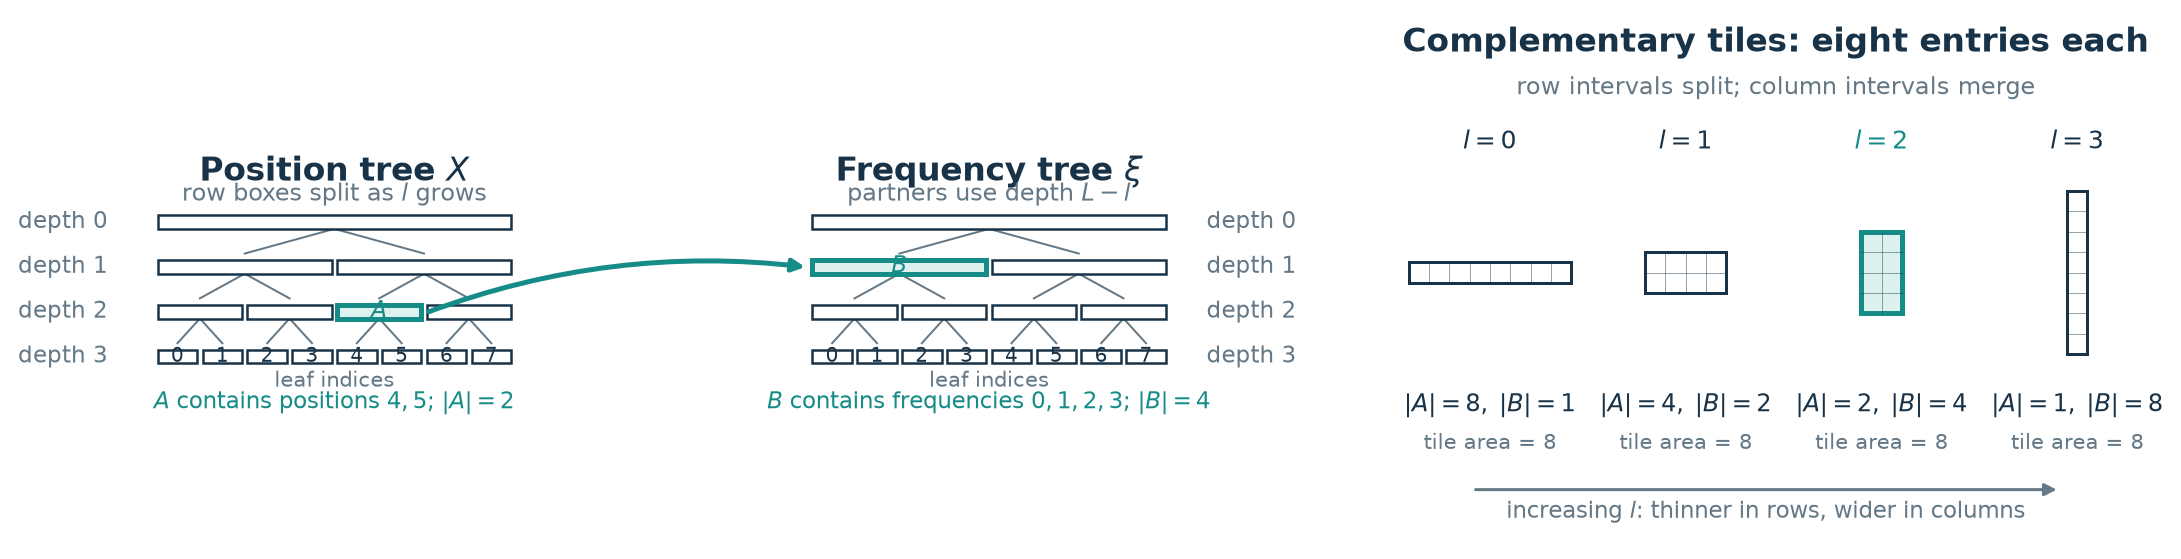
\includegraphics[width=\linewidth]{figures/two-trees.png}
\caption{Two dyadic trees and complementary tilings at $N=8$. The selected pair has depths $\ell=2$ and $L-\ell=1$. Row intervals split with depth while their column partners merge; each displayed tile has eight entries with a different aspect ratio.}
\label{fig:two-trees}
\end{figure}

In the bilinear example,~\eqref{eq:constant-residual} implies that the same $q$ in~\eqref{eq:bilinear-exponential} gives the same local error bound at every level. In the analytic theorem, the hypotheses hold on every complementary pair, so its rank bound is also uniform over the ladder. Near the middle level, both widths are approximately $n^{-1/2}$. This is where the algorithm changes from interpolation in the source variable to interpolation in the observation variable, always choosing the smaller box.

The word \emph{local} matters. A uniform error on every block does not, by itself, bound the error of the complete multilevel recursion; propagated errors must also be tracked. The geometric estimate explains why no level intrinsically requires a larger rank than another.

\subsection{From low-rank blocks to the butterfly recursion}
\label{subsec:butterfly-recursion}

For any source box $B$, define the partial potential
\begin{equation}
    u_B(x)=\sum_{p_j\in B}K_n(x,p_j)f(p_j).
\end{equation}
A rank-$r$ approximation on $A\times B$,
$K_n(x,p)\approx\sum_{t=1}^{r}\alpha_t^{AB}(x)\beta_t^{AB}(p)$, reduces this potential on $A$ to
\begin{equation}
    u_B(x)\approx\sum_{t=1}^{r}\alpha_t^{AB}(x)\delta_t^{AB},
    \qquad
    \delta_t^{AB}=\sum_{p_j\in B}\beta_t^{AB}(p_j)f(p_j).
    \label{eq:compressed-potential}
\end{equation}
Only $r$ coefficients are needed to describe the contribution of $B$ throughout $A$.

The butterfly algorithm avoids calculating these coefficients independently from all the sources in every large box. At the next level, $A$ is replaced by one of its children and $B$ by its parent. The approximations already available on the parent of $A$ and the children of $B$ are recombined, after which the new complementary low-rank representation compresses them again. Thus short coefficient vectors are transferred through the levels by small matrices. At the last level, $B$ is the whole source domain and~\eqref{eq:compressed-potential} is evaluated on each observation leaf.

At a fixed level of the one-dimensional ladder, there are $2^\ell$ observation boxes and $2^{L-\ell}$ source boxes, hence $2^L=n$ complementary pairs. Across the $L+1$ levels this gives $O(n\log n)$ pairs. If the rank is fixed, the work per pair is also fixed, so the recursive updates cost $O(n\log n)$. In the paper's two-dimensional quadtree construction, let $N_{\mathrm{pd}}$ denote the per-dimension grid parameter, so there are $N_{\mathrm{tot}}=N_{\mathrm{pd}}^2$ unknowns. The same count gives $N_{\mathrm{pd}}^2$ pairs per level and $O(N_{\mathrm{pd}}^2\log N_{\mathrm{pd}})$ pairs in total. For fixed tolerance, the operation count is thus $O(N_{\mathrm{pd}}^2\log N_{\mathrm{pd}})=O(N_{\mathrm{tot}}\log N_{\mathrm{tot}})$.

These counts concern the explicit-kernel butterfly traversal and application, not the separate task of constructing a general butterfly factorization from a matrix alone. For the matrix-side construction of Li et al., with $N_{\mathrm{tot}}$ the matrix dimension, applying the resulting sparse factors costs $O(N_{\mathrm{tot}}\log N_{\mathrm{tot}})$. Their construction costs $O(N_{\mathrm{tot}}^{3/2})$ when blocks are sampled directly, or $O(C_K(N_{\mathrm{tot}})\sqrt{N_{\mathrm{tot}}}+N_{\mathrm{tot}}^{3/2})$ using black-box applications of the matrix and its adjoint, where $C_K(N_{\mathrm{tot}})$ is one such application. When $C_K(N_{\mathrm{tot}})=O(N_{\mathrm{tot}}\log N_{\mathrm{tot}})$, the latter becomes $O(N_{\mathrm{tot}}^{3/2}\log N_{\mathrm{tot}})$. These are different algorithms and should not be conflated.

\subsection{The complementary low-rank condition}
\label{subsec:complementary-low-rank}

The same structure can be described entirely in matrix language. Let $K$ be a matrix whose row and column indices are organized by trees $T_X$ and $T_P$ of depth $L$. It satisfies the \emph{complementary low-rank property} if, for a prescribed absolute spectral tolerance $\varepsilon$, every block
\begin{equation}
    K_{A,B},\qquad A\in T_X,\quad B\in T_P,
    \quad \ell(A)+\ell(B)=L,
\end{equation}
can be approximated to this accuracy in spectral norm with rank at most $r_\varepsilon$, where $r_\varepsilon$ is small compared with the matrix dimensions. General butterfly factorizations assume this property and convert the collection of block approximations into a product of sparse factors~\cite{li2015butterfly}.

For uniformly refined square boxes, $\ell(A)+\ell(B)=L$ means that $h_Ah_B$ is of order $2^{-L}$. In the FIO normalization above, this is exactly $1/n$. The centered expansion therefore supplies an analytic explanation for the complementary low-rank assumption: the double difference contains only mixed derivatives, and the width-product condition bounds the residual phase uniformly. For the analytic FIOs considered here, the theorem quoted above verifies the required rank bound.

This is not the usual statement that only well-separated, off-diagonal blocks are low rank. Complementary pairs cover the whole matrix, including geometrically close boxes; the saving comes from replacing every such block by a short separated expansion, not from discarding interactions. Nor is the property automatic for every oscillatory or Green-function matrix. Smoothness of the transformed phase and the validity of the width-product estimate are essential.

Finally, we relate the notation to the original paper. Cand\`{e}s--Demanet--Ying consider two-dimensional operators with a phase $\Phi(x,k)$ homogeneous of degree one in $k$. The polar rescaling $k=(N/\sqrt2)\,p_1v(p_2)$, where $v(p_2)=(\cos 2\pi p_2,\sin 2\pi p_2)$, gives $\Phi(x,k)=N\Psi(x,p)$ with $\Psi(x,p)=\Phi(x,v(p_2))p_1/\sqrt2$. Thus the kernel becomes $e^{2\pi i N\Psi(x,p)}$ with $x,p\in[0,1]^2$. Their square boxes satisfy $w(A)w(B)=1/N$, which is the two-dimensional counterpart of~\eqref{eq:ladder-widths}. Thus the one-dimensional calculation above isolates the central idea without changing its geometric content.

% SECTION 5: synthesis of the matrix-side and experimental material.
\section{Numerical linear algebra and computational evidence}
\label{sec:numerical-evidence}

Section~\ref{sec:butterfly} derives local compressibility from the phase and describes the coefficient recursion. We now make the global algebra explicit: first the original algorithm's two online invariants, then a target-only alternative with one invariant, its interpolative-decomposition extension, and controlled computational checks. Unless stated otherwise, $N$ in this section is the total matrix dimension, not the per-dimension parameter $N_{\mathrm{pd}}$ used for the two-dimensional quadtree above. Construction cost, solve diagnostics, and physical accuracy remain separate questions throughout.

\subsection{Local rank is not yet a fast algorithm}
Consider the middle level of two binary index trees of depth $L=\log_2N$, with $L$ even. There are $N$ complementary square tiles of size $\sqrt N\times\sqrt N$. If each has rank at most $r$, storing independent low-rank factors takes
\begin{equation}
 N\times O(r\sqrt N)=O(rN^{3/2})
 \label{eq:middlecost}
\end{equation}
leading entries. This is already different from dense storage, but it is not $O(N\log N)$: there are too many unrelated bases. Computing those factors by reading every tile also costs at least $\Theta(N^2)$ entry accesses.

Nesting removes the first obstruction. Suppose old summaries $c_1,c_2$ contribute to a new tile whose basis is $U_{\rm new}$:
\begin{equation}
 U_1c_1+U_2c_2
 \approx U_{\rm new}(T_1c_1+T_2c_2).
 \label{eq:transfer}
\end{equation}
The small matrices $T_1,T_2$ reuse earlier coefficients rather than recomputing them from sources. If the old ranks are $r_0,r_1$ and the new rank is $r_2$, a merge stores at most $r_2(r_0+r_1)$ entries before zero and identity entries are removed. With bounded ranks, $O(N)$ entries per stage and $O(\log N)$ stages give $O(N\log N)$ storage and apply work~\cite{li2015butterfly}.
\takeaway{Complementary tiles supply local rank; nesting supplies global speed.}

This is the matrix-side counterpart of the compressed-potential recursion~\eqref{eq:compressed-potential}. It also distinguishes two operations that are easy to conflate: applying stored sparse factors is cheap, while constructing them may dominate. Direct entry access, black-box products with $K$ and $K^*$, and entry-sampled constructors have different costs and hypotheses. The detailed estimates stated at the end of Section~\ref{subsec:butterfly-recursion} must therefore be attached to the corresponding constructor rather than quoted as one universal ``butterfly complexity.''

\subsection{The DFT is the exact rank-one special case}
The centered phase expansion in Section~\ref{sec:butterfly} is approximate for a general phase. For the DFT, an exact residue identity makes the same tiling rank one. Let $\widetilde F_N=\sqrt N\,\mathcal F_N$, so $(\widetilde F_N)_{jk}=e^{-2\pi ijk/N}$. Choose residue classes
\[
 j=a+2^\ell u,\qquad k=b+2^{L-\ell}v.
\]
Then
\begin{equation}
 \frac{jk}{N}=\frac{ab}{N}+\frac{av}{2^\ell}
 +\frac{bu}{2^{L-\ell}}+uv .
 \label{eq:residue-identity}
\end{equation}
Since $uv\in\mathbb Z$, $e^{-2\pi iuv}=1$. The block therefore factors into a constant, a row-only vector, and a column-only vector, so its exact rank is one. Matched bit reversal makes these residue classes contiguous in both trees. Reversing only one tree does not create this identity; Section~2's global full-rank obstruction and the present block rank-one statement are compatible because they concern different index sets.

For the explicit rank-one factor representation used in the supplement, the number of stored entries is
\begin{equation}
 \nnz=2N\log_2N+2N .
 \label{eq:fftcount}
\end{equation}
This is not the memory requirement of an in-place FFT, nor is it the same sparse-stage convention as~\eqref{eq:fft-stages}. It is a count for one explicit butterfly-style factor chain. The included Rust example independently checks rank-one tiles, reconstruction, and this entry count~\cite{li2015butterfly}.
\begin{evidence}
Equation~\eqref{eq:residue-identity} proves exact rank one for every complementary residue block. The storage count is proved by summing the named factor sizes. Recorded package checks and their current rerun status are listed in Appendix~\ref{app:verification}.
\end{evidence}

\subsection{The original algorithm through two online invariants}
\label{sec:two-invariants}

The nesting relation~\eqref{eq:transfer} tells us that small transfers exist, but not what their intermediate coefficients mean. The middle-seeded construction of Li et al. becomes clearer when those meanings are stated as invariants~\cite{li2015butterfly}. Let $K\in\mathbb C^{N\times N}$, $N=2^L$, and let $A_i^\ell$ and $B_j^{L-\ell}$ be dyadic row and column nodes at complementary depths. Write
\begin{equation}
 K_{ij}^{\ell}:=K[A_i^\ell,B_j^{L-\ell}],
 \qquad g_j^\ell:=g[B_j^{L-\ell}],
 \qquad 0\le i<2^\ell,\quad 0\le j<2^{L-\ell}.
 \label{eq:invariant-block}
\end{equation}
There are $N$ slots $(i,j)$ at each level. The middle level is $h=L/2$, with square blocks of size $\sqrt N\times\sqrt N$. Start from local approximations
\begin{equation}
 K_{ij}^h\simeq P_{ij}^hC_{ij}^h(Q_{ij}^h)^*,
 \qquad P^*P=Q^*Q=I,
 \label{eq:invariant-seed}
\end{equation}
where $C$ is small and, for an SVD seed, diagonal.

On the source half, a slot stores coordinates of the input band:
\begin{equation}
 z_{ij}^{t}\approx(Q_{ij}^{t})^*g_j^t,
 \qquad 0\le t\le h.
 \label{eq:source-invariant}
\end{equation}
For a destination slot $(i',j')$ at level $t$, put $i=\lfloor i'/2\rfloor$, $a=(i,2j')$, and $b=(i,2j'+1)$. Because the new input band is the concatenation of the two old bands,
\begin{equation}
 z_{i'j'}^t=F_{i'j'}^t
 \begin{bmatrix}z_a^{t-1}\\z_b^{t-1}\end{bmatrix},
 \qquad
 F_{i'j'}^t=(Q_{i'j'}^t)^*
 \begin{bmatrix}Q_a^{t-1}&0\\0&Q_b^{t-1}\end{bmatrix}.
 \label{eq:source-transfer}
\end{equation}
At the middle, multiplication by $C_{ij}^h$ changes the meaning of the state without combining different matrix blocks:
\begin{equation}
 w_{ij}^h:=C_{ij}^hz_{ij}^h,
 \qquad
 P_{ij}^hw_{ij}^h\approx K_{ij}^hg_j^h.
 \label{eq:middle-handoff}
\end{equation}
The second invariant, now valid for the output half, is
\begin{equation}
 \boxed{\;P_{ij}^{\ell}w_{ij}^{\ell}\approx K_{ij}^{\ell}g_j^{\ell}\;}.
 \label{eq:target-invariant}
\end{equation}
Thus the left side represents one block's contribution to the output, not input coordinates. Summing these contributions over $j$ for fixed $i$ gives the answer on $A_i^\ell$.

To preserve~\eqref{eq:target-invariant} at level $\ell+1$, let $R_{i'}$ restrict to a row child and define
\begin{equation}
 G_{i'j'}^\ell=(P_{i'j'}^{\ell+1})^*
 \begin{bmatrix}R_{i'}P_a^\ell&R_{i'}P_b^\ell\end{bmatrix},
 \qquad
 w_{i'j'}^{\ell+1}=G_{i'j'}^\ell
 \begin{bmatrix}w_a^\ell\\w_b^\ell\end{bmatrix}.
 \label{eq:target-transfer}
\end{equation}
With $\Pi_{i'j'}^{\ell+1}=P_{i'j'}^{\ell+1}(P_{i'j'}^{\ell+1})^*$, substitution gives
\begin{align}
 P_{i'j'}^{\ell+1}w_{i'j'}^{\ell+1}
 &=\Pi_{i'j'}^{\ell+1}R_{i'}(P_a^\ell w_a^\ell+P_b^\ell w_b^\ell)\\
 &\approx\Pi_{i'j'}^{\ell+1}R_{i'}(K_a^\ell g_a^\ell+K_b^\ell g_b^\ell)
 =\Pi_{i'j'}^{\ell+1}K_{i'j'}^{\ell+1}g_{j'}^{\ell+1}.
 \label{eq:target-proof}
\end{align}
Restriction and addition over disjoint bands are exact; the displayed projection is the new local truncation. Two parent matrices therefore feed each of two child matrices, rather than there being a global two-to-one reduction. At $\ell=L$, row nodes are singletons and the invariant gives the desired approximation to $Kg$.

The balanced seed is an offline device. Sampling $O(\rho_\ell)$ rows and columns of all $N$ level-$\ell$ blocks, with $\rho_\ell$ the local coordinate bound, costs
\[
 O\!\left(N\rho_\ell\left(\frac{N}{2^\ell}+2^\ell\right)\right)
\]
entry accesses up to local decomposition constants. At fixed rank, the factor in parentheses is minimized near $2^\ell=\sqrt N$. This is the construction-side reason for starting in the middle, not an additional online approximation principle. If each transfer has rank product at most $r^2$, the $N$ slots per level and $L$ levels give
\begin{equation}
 O(Nr^2\log N)
 \label{eq:online-transfer-cost}
\end{equation}
application work and sparse-transfer storage. The middle coupling and terminal diagonal initialization do not change this order.

\subsection{A target-only alternative with one invariant}
\label{sec:target-only}

The original online sweep has input coordinates before the middle and output contributions afterwards. A middle-seeded alternative keeps~\eqref{eq:target-invariant} at every level. Formally, its factor chain is
\begin{equation}
 K\approx U^LG^{L-1}\cdots G^0D.
 \label{eq:target-only-chain}
\end{equation}
At level zero, one could explain the initialization by normalizing each full column $k_j=K[:,j]$: $P_{0j}^0=k_j/\|k_j\|_2$, $D_{jj}=\|k_j\|_2$, and $w_{0j}^0=D_{jj}g_j$, with an arbitrary unit basis for a zero column. This makes $P_{0j}^0w_{0j}^0=k_jg_j$ exact. The formula explains the invariant; it is not the implemented constructor, because reading and normalizing all full columns would itself require $\Theta(N^2)$ entry accesses.

The constructor starts from the same middle representation as the original algorithm. Write a represented middle block as
\[
 \widetilde K_{ij}^h=P_{ij}^hW_{ij}^h,
 \qquad W_{ij}^h=C_{ij}^h(Q_{ij}^h)^*.
\]
Suppose finer represented blocks are known as $P_{ij}^{\ell+1}W_{ij}^{\ell+1}$. For a coarse slot $(i,j)$, put $\widehat\jmath=\lfloor j/2\rfloor$. Let $S_j$ select the columns of the fine band belonging to child $B_j^{L-\ell}$, and form the small stacked coefficient matrix
\begin{equation}
 \mathcal U_{ij}^{\ell}:=
 \begin{bmatrix}
 W_{2i,\widehat\jmath}^{\ell+1}S_j\\[2pt]
 W_{2i+1,\widehat\jmath}^{\ell+1}S_j
 \end{bmatrix}
 \approx\mathcal Q_{ij}^{\ell}W_{ij}^{\ell},
 \label{eq:small-qr}
\end{equation}
using reduced pivoted QR (or an SVD), with truncation only when requested. The new represented basis and coarse block are
\begin{equation}
 P_{ij}^{\ell}:=
 \begin{bmatrix}P_{2i,\widehat\jmath}^{\ell+1}&0\\0&P_{2i+1,\widehat\jmath}^{\ell+1}\end{bmatrix}
 \mathcal Q_{ij}^{\ell},
 \qquad
 \widetilde K_{ij}^{\ell}=P_{ij}^{\ell}W_{ij}^{\ell}.
 \label{eq:coarse-target-basis}
\end{equation}
Direct substitution into the vertical block identity justifies this relation. If the small QR is exact, the represented coarse block is exact; if it is truncated, the discarded term is visible in~\eqref{eq:small-qr}. The large product in~\eqref{eq:coarse-target-basis} need not be formed.

For an online destination $(i',j')$, let $c\in\{0,1\}$ select its child-row half of $\mathcal Q$. The transfer in~\eqref{eq:target-transfer} reduces to the top or bottom row half of two small $\mathcal Q$ matrices:
\begin{equation}
 G_{i'j'}^\ell=
 \begin{bmatrix}(\mathcal Q_{i,2j'}^\ell)_c&(\mathcal Q_{i,2j'+1}^\ell)_c\end{bmatrix}.
 \label{eq:qr-target-transfer}
\end{equation}
Repeating the descent for $\ell=h-1,\ldots,0$ produces all coarse online transfers. At level zero only $D=W^0$ and the small transfers are stored; normalized full-column bases remain implicit. No additional entries of $K$ are read during this coefficient descent. With local ranks bounded by $r$, its level-$\ell$ work is $O(Nr^22^\ell)$, hence
\begin{equation}
 \sum_{\ell=0}^{h-1}O(Nr^22^\ell)=O(N^{3/2}r^2).
 \label{eq:qr-descent-cost}
\end{equation}
This cost excludes the common middle seed and upper target construction. The online order remains~\eqref{eq:online-transfer-cost}. The simplification is therefore a single partial-product invariant and a smaller organizational constant, not a new asymptotic application rate.
\begin{evidence}
Equations~\eqref{eq:small-qr}--\eqref{eq:qr-target-transfer} prove the construction for each represented block by substitution. They do not supply an unconditional global error theorem after truncated middle data and local compressions; those errors still need propagation analysis.
\end{evidence}

\subsection{Extension to original-column interpolative bases}
\label{sec:idbf-target}
Interpolative decomposition butterfly factorization (IDBF) replaces orthonormal projections by selected original columns~\cite{pang2018idbf}. A column ID of $B$ is $B\approx B[:,q]V$, where $q$ selects columns and $V$ interpolates the rest. Define an output basis
\begin{equation}
 P_{ij}^{\ell}=K[A_i^\ell,q_{ij}^{\ell}],
 \label{eq:id-original-basis}
\end{equation}
where $q_{ij}^{\ell}$ is a short list of global columns in $B_j^{L-\ell}$. The partial-product invariant remains~\eqref{eq:target-invariant}. Instead of the orthonormal transfer, form
\begin{equation}
 \mathcal B_{i'j'}^{\ell}:=
 \begin{bmatrix}R_{i'}P_a^\ell&R_{i'}P_b^\ell\end{bmatrix}
 \approx P_{i'j'}^{\ell+1}G_{i'j'}^\ell,
 \qquad
 P_{i'j'}^{\ell+1}:=(\mathcal B_{i'j'}^\ell)[:,p].
 \label{eq:id-target-transfer}
\end{equation}
The online update is again $w_{i'j'}^{\ell+1}=G_{i'j'}^\ell[w_a^\ell;w_b^\ell]$, and the projection proof~\eqref{eq:target-proof} is unchanged except that the new local residual is a column-ID residual. Since selected candidates are original columns, the new index list is a subset of the two parent lists.

Under the standard IDBF sampled-ID assumptions, sampling $O(k)$ rows of a candidate with $O(k)$ columns costs $O(k^3)$ per slot. The usual IDBF slot counts then give construction $O(k^3N\log N/n_0)$ and online storage/application $O(k^2N\log N/n_0)$ for leaf size $n_0$. This is a conditional mathematical construction, not the access pattern of the visible-entry prototype below. Sampled rows must reveal the range, interpolation coefficients must be controlled, and local residuals still accumulate.

For a controlled two-sided comparison, a middle block can be normalized through row and column IDs as
\begin{equation}
 K_{ij}^h\approx U_{ij}R_{ij}
 \approx (U_{ij}S_{ij})S_{ij}^{-1}R_{ij}
 =P_{ij}^hW_{ij}^h,
 \qquad W_{ij}^h=V_{ij}.
 \label{eq:id-shared-seed}
\end{equation}
Here $P_{ij}^h$ consists of selected original columns up to ID residuals, $S_{ij}$ is the small cross skeleton, and its inverse is computed only offline. The original-style branch stores selected-row coordinates before multiplication by $S_{ij}^{-1}$ and output contributions afterwards. The target-only branch uses original-column cIDs throughout. Both receive the same middle data and upper factors in the implementation comparison.

\subsection{Controlled checks of the target-only construction}
\label{sec:target-only-checks}
The scripts in \path{examples/target-only/} implement both variants on the exact-rank oracle
\[
 K=\frac1{\sqrt{Nr}}AB^*,
 \qquad A,B\in\mathbb C^{N\times r},\qquad r=4,
\]
with deterministic standard complex Gaussian entries. Every complementary block thus has exact rank at most four. This deliberately isolates differences in online organization from approximation-tolerance differences. The SVD comparison uses common literal middle SVDs; the IDBF comparison uses common two-sided deterministic IDs. Applications use one BLAS/OpenMP thread and medians of repeated batches.

Table~\ref{tab:target-only-results} reports locally rerun application ratios and structural online entry counts. ``Original'' means input/source coordinates followed by the middle coupling and output factors; ``target'' means one partial-product chain. The entry counts include transfers, terminal blocks, initialization data, and the original middle coupling where applicable.
\begin{table}[htbp]
\centering\small
\caption{Local checks at exact rank four: application ratio original/target (above one means target is faster), structural complex-entry counts, and mutual output error. Times are medians on this VM, not portable speedup guarantees.}
\label{tab:target-only-results}
\begin{tabular}{@{}lrrrr@{}}
\toprule
$N$ & Application ratio & Original entries & Target entries & Mutual error\\
\midrule
\multicolumn{5}{@{}l@{}}{\emph{SVD middle seed: source $+M^h$ versus target-only QR descent}}\\
16  & $1.033$ & $736$    & $672$    & $6.62\times10^{-16}$\\
64  & $1.016$ & $7040$   & $6784$   & $1.06\times10^{-15}$\\
256 & $1.002$ & $44544$  & $43520$  & $1.50\times10^{-15}$\\
\addlinespace
\multicolumn{5}{@{}l@{}}{\emph{Two-sided IDBF seed: source $+C^h$ versus target-only cIDs}}\\
16  & $1.116$ & $912$    & $656$    & $1.27\times10^{-15}$\\
64  & $1.090$ & $7744$   & $6720$   & $1.59\times10^{-15}$\\
256 & $1.068$ & $47360$  & $43264$  & $2.56\times10^{-15}$\\
\bottomrule
\end{tabular}
\end{table}

For the SVD form, unshared source/target construction ratios were $1.679$, $1.693$, and $1.771$ at $N=16,64,256$. Including the common literal-SVD seed and upper factors reduced the corresponding setup ratios to $1.154$, $1.202$, and $1.193$. Four random complex inputs at $N=16,64$ gave worst absolute-reference relative errors below $1.8\times10^{-15}$ for both applications.

For IDBF, unshared source/target construction ratios were $2.570$, $3.091$, and $3.067$. At $N=16,64,256$, four-input original/target errors were at most $2.16\times10^{-15}$ and $1.63\times10^{-15}$, respectively. Independent coordinate-vector checks reconstructed the dense operators at the same scale, and the target partial-product identity held at every slot and level with worst normalized errors $2.23\times10^{-15}$, $5.40\times10^{-15}$, and $1.40\times10^{-14}$.
\begin{evidence}
These are locally regenerated computations on exact-rank matrices at the three displayed sizes. They support the implemented invariant and measured constant-factor differences for this prototype. They do not test nontrivial approximation ranks, a production sparse kernel, or optimized sampled-entry construction. Full setup costs and common-seed costs are kept separate from online application timings.
\end{evidence}

\subsection{An apply factorization does not certify elimination}
A second matrix-side distinction appears in direct solvers. Suppose an interpolative decomposition has produced a relation between redundant and skeleton unknowns. A row operation must then be implemented with the correct adjoint, not merely with a convenient transpose.

For a concrete mechanism, let $\Pi=[I;-T]$ and suppose the Hermitian part of $W$ satisfies $\operatorname{Herm}(W)\succeq\mu I$ with $\mu>0$. The adjoint row operation gives the congruence
\begin{equation}
 \operatorname{Herm}(\Pi^*W\Pi)
 =\Pi^*\operatorname{Herm}(W)\Pi
 \succeq\mu(I+T^*T)\succeq\mu I .
 \label{eq:adjoint-congruence}
\end{equation}
Replacing $\Pi^*$ by the ordinary complex transpose $\Pi^{\T}$ destroys this argument: in the scalar case $W=1$ and $T=i$, one obtains $\Pi^{\T}\Pi=1+i^2=0$, whereas $\Pi^*\Pi=2$. An accurate compressed apply therefore leaves a separate pivot-stability question in a complex elimination. This identity is proved here; the frequency-dependent numerical consequences are experimental, not a universal theorem about every FMM-LU implementation.

\subsection{A numerical check using the discrete Fourier transform}
\label{subsec:butterfly-dft-demo}

The bilinear case gives a direct numerical check. Take $N$ observation and source points $x_i=i/N$ and $p_j=j/N$, where $i,j=0,\ldots,N-1$. Then
\begin{equation}
    e^{2\pi i N\Psi(x_i,p_j)}
    =e^{2\pi i ij/N},
\end{equation}
so $\Psi(x,p)=xp$ gives the positive-sign discrete Fourier transform. NumPy's default inverse FFT includes the normalization $1/N$:
\begin{equation}
    \operatorname{IFFT}(f)_i
    =\frac1N\sum_{j=0}^{N-1}e^{2\pi i ij/N}f_j.
\end{equation}
Consequently $u=N\,\operatorname{IFFT}(f)$ is the desired positive-sign transform, computed exactly up to floating-point roundoff.

Figure~\ref{fig:butterfly-dft-demo} compares this reference with the centered-residual algorithm. The implementation is provided in \path{examples/butterfly/}. The Taylor calculation above is an error model; the implementation instead uses Chebyshev interpolation of the residual exponential, as described earlier. Increasing $q$ rapidly decreases the approximation error. The top-right panel explicitly plots this error against $N$: at fixed $q=8$ it remains approximately constant over the tested sizes. The implementation performs $N$ complementary paired updates at each level, and the timing panel includes both an $N\log N$ guide and an $N^2$ guide. Wall time is not the main comparison: the FFT is an optimized algorithm specialized to this transform, whereas the Python butterfly code is a minimal demonstration. These numerical checks are empirical; they are not a proof of a global error bound.

\begin{figure}[htbp]
    \centering
    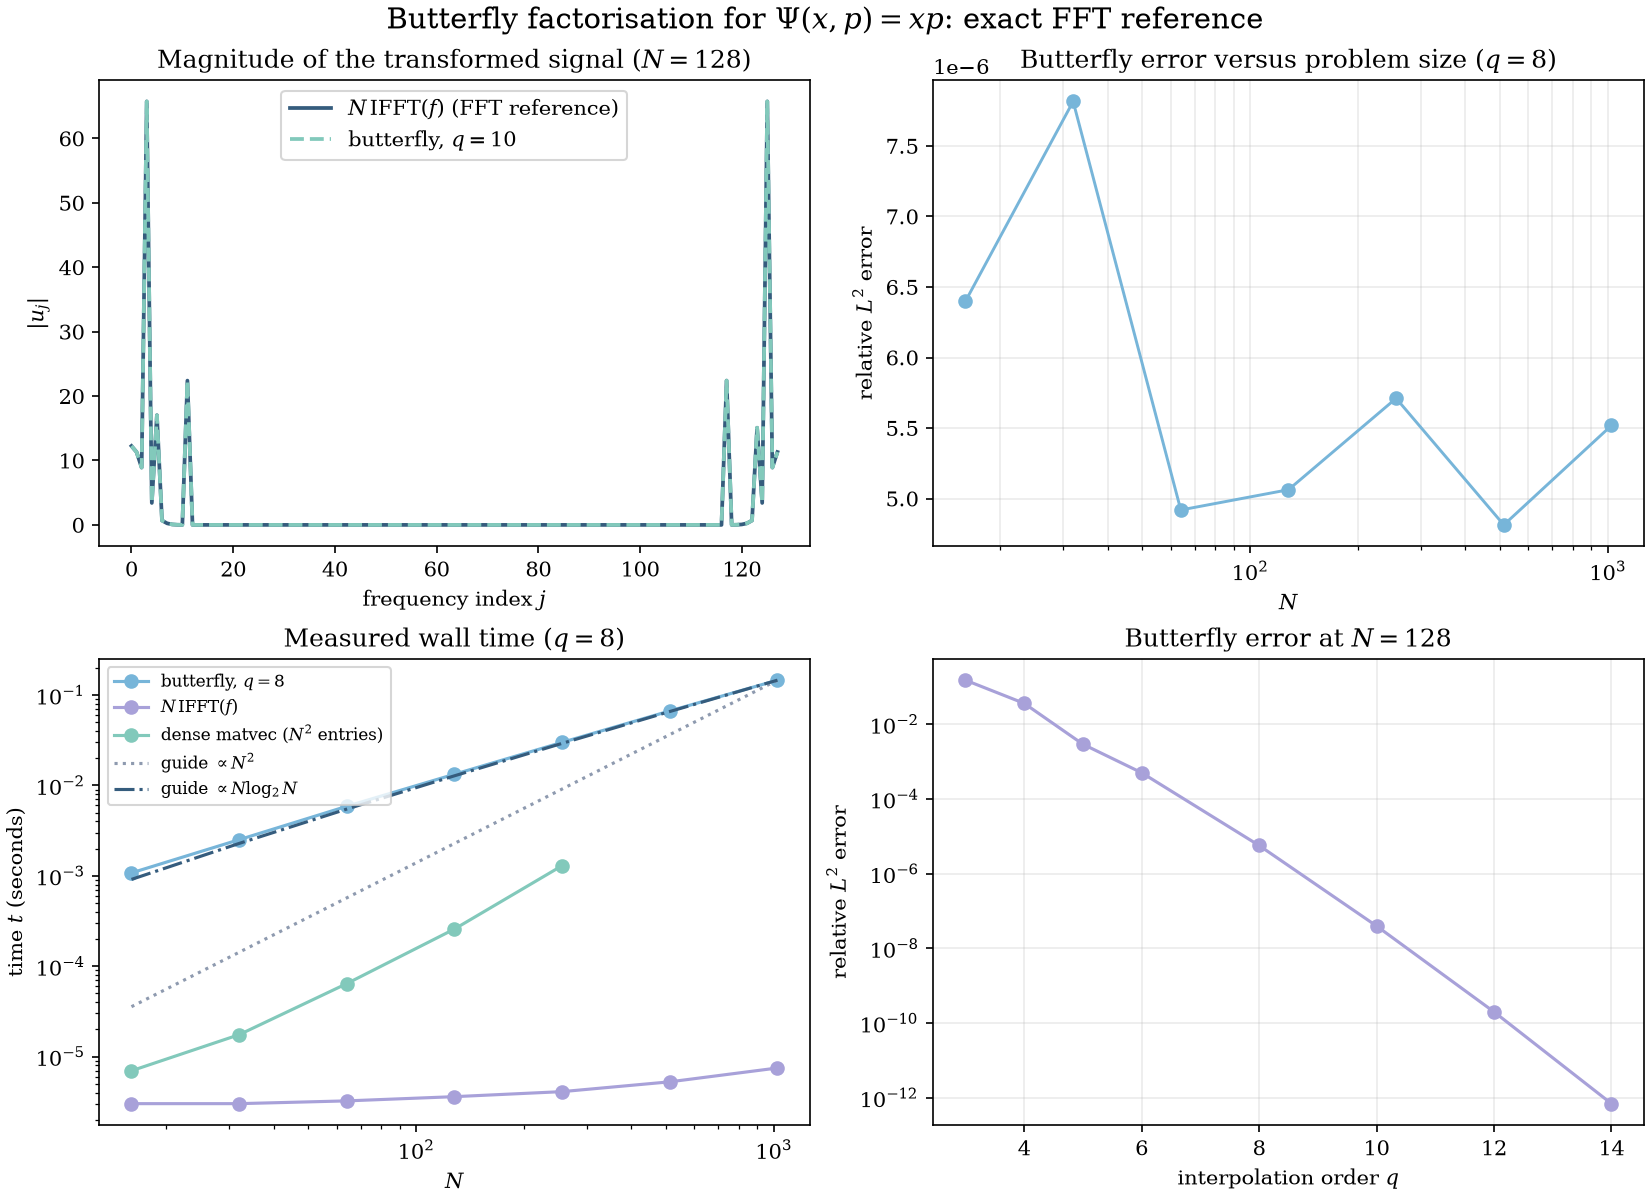
\includegraphics[width=\textwidth]{figures/butterfly-dft.png}
    \caption{Comparison of the butterfly algorithm with the exact FFT reference for $\Psi(x,p)=xp$. \emph{Top left:} transformed magnitudes for a complex test signal at $N=128$, using $q=10$; the two curves are nearly indistinguishable. \emph{Top right:} relative Euclidean output error versus $N$ at fixed $q=8$, shown separately from the dependence on $q$. \emph{Bottom left:} single-thread wall times at $q=8$ for $N=16,\ldots,1024$, including a dense matrix--vector product for $N\leq256$ and guides proportional to $N\log_2N$ and $N^2$. The dense path was warmed up before timing; absolute times are machine dependent. \emph{Bottom right:} relative $L^2$ error $\|u_q-u_{\mathrm{FFT}}\|_2/\|u_{\mathrm{FFT}}\|_2$ at $N=128$ as the Chebyshev interpolation order $q$ varies. All approximation errors use $u_{\mathrm{FFT}}=N\,\operatorname{IFFT}(f)$ as the reference.}
    \label{fig:butterfly-dft-demo}
\end{figure}

\subsection{A non-DFT oscillatory example}
\label{subsec:non-dft-demo}

To check that the construction is not tied to the Fourier transform, consider
\begin{equation}
    \Psi(x,p)=xp+0.1x^2p^2.
    \label{eq:non-dft-phase}
\end{equation}
This is still real-analytic, but $R_{AB}$ is no longer simply $(x-a)(p-b)$. The explicit Taylor estimate for the bilinear example therefore does not apply; the local approximation is constructed by residual interpolation.

Figure~\ref{fig:non-dft-demo} uses this phase in the same implementation, now comparing against an explicit dense evaluation of
$Kf$, not against an FFT. The transformed magnitudes at $q=10$ agree closely, and increasing $q$ again rapidly reduces the relative Euclidean output error. This is an additional numerical test of the approximation, not a claim of a global diagonalisation or a global error estimate.

\begin{figure}[htbp]
    \centering
    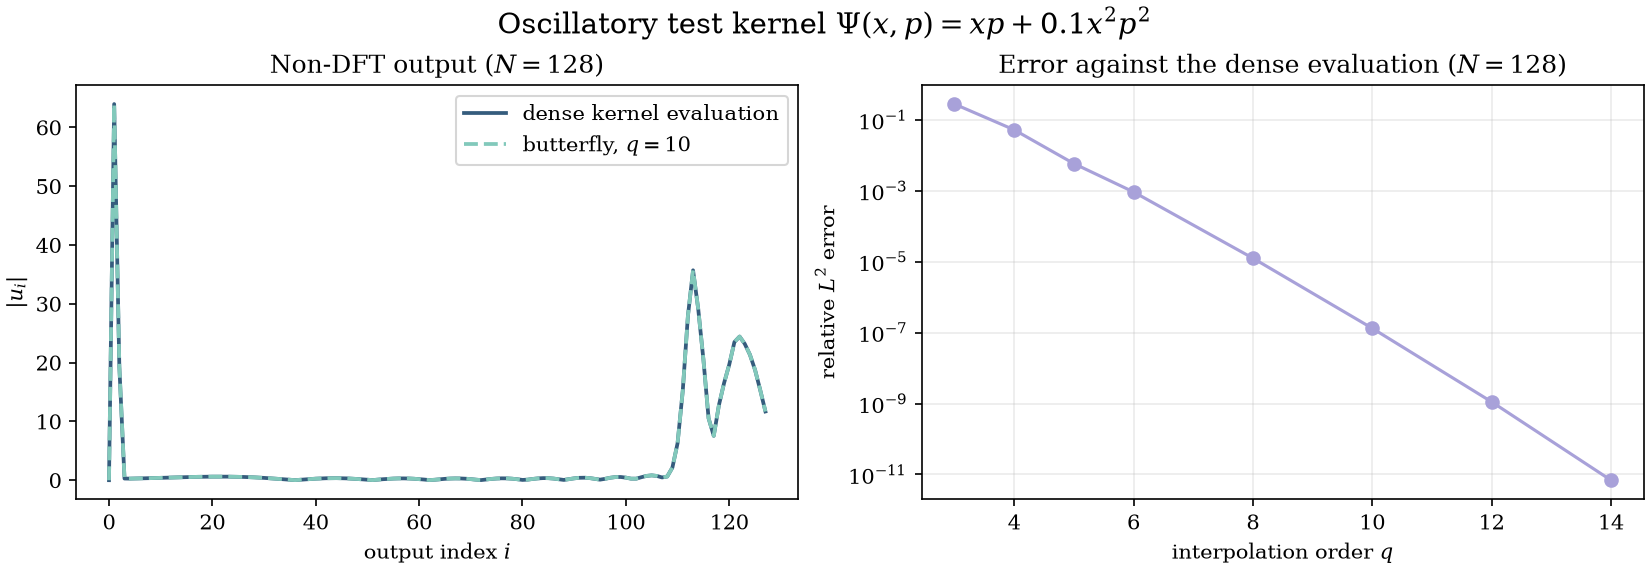
\includegraphics[width=\textwidth]{figures/butterfly-non-dft.png}
    \caption{Application to the non-DFT oscillatory test kernel $\Psi(x,p)=xp+0.1x^2p^2$ at $N=128$. \emph{Left:} output magnitudes from the explicit dense kernel evaluation and from the butterfly algorithm at $q=10$. \emph{Right:} relative $L^2$ error $\|u_q-u_{\mathrm{dense}}\|_2/\|u_{\mathrm{dense}}\|_2$ against the Chebyshev interpolation order $q$. Unlike the DFT comparison, the reference here is computed entirely by dense evaluation of~\eqref{eq:non-dft-phase}.}
    \label{fig:non-dft-demo}
\end{figure}

\subsection{Local reproduction: two oscillatory kernels}
The code in \path{examples/butterfly/} implements one-dimensional residual interpolation and nested transfers without forming an $N\times N$ matrix in the butterfly apply. The DFT reference is the positive-sign transform
\begin{equation}
 u_i=\sum_{j=0}^{N-1}e^{2\pi iij/N}f_j
 =N\,\operatorname{IFFT}(f)_i,
 \label{eq:positive-dft}
\end{equation}
where the sign differs deliberately from the unitary negative-sign convention in Section~\ref{sec:fft}. The non-DFT reference is a dense evaluation of the phase~\eqref{eq:non-dft-phase}.

Table~\ref{tab:butterfly-accuracy} gives locally regenerated results at $N=128$ for one deterministic complex input in the DFT case and for $f_j=\sin(2\pi j/N)+0.3i\cos(4\pi j/N)$ in the non-DFT case. Here $q$ is the residual's Chebyshev--Lobatto interpolation order in each one-dimensional interpolation direction.
\begin{table}[htbp]
\centering\small
\caption{Locally rerun relative Euclidean output errors at $N=128$. The two columns use different references: $N\,\operatorname{IFFT}(f)$ for $\Psi=xp$ and explicit dense kernel evaluation for $\Psi=xp+0.1x^2p^2$.}
\label{tab:butterfly-accuracy}
\begin{tabular}{@{}rrr@{}}
\toprule
$q$ & DFT phase & Non-DFT phase \\
\midrule
3  & $1.506\times10^{-1}$ & $2.785\times10^{-1}$\\
4  & $3.609\times10^{-2}$ & $5.228\times10^{-2}$\\
5  & $2.905\times10^{-3}$ & $5.838\times10^{-3}$\\
6  & $5.009\times10^{-4}$ & $9.271\times10^{-4}$\\
8  & $5.652\times10^{-6}$ & $1.256\times10^{-5}$\\
10 & $3.950\times10^{-8}$ & $1.324\times10^{-7}$\\
12 & $1.983\times10^{-10}$ & $1.116\times10^{-9}$\\
14 & $6.920\times10^{-13}$ & $6.879\times10^{-12}$\\
\bottomrule
\end{tabular}
\end{table}

At fixed $q=8$, a second sweep over $N=16,32,\ldots,1024$ gave relative errors between $4.81\times10^{-6}$ and $7.82\times10^{-6}$. The complementary pair counts matched $N(\log_2N+1)$ exactly, rising from $80$ at $N=16$ to $11{,}264$ at $N=1024$. Four unit tests pass locally: FFT/dense agreement, DFT butterfly convergence, fixed-$q$ error stability over $N=16,32,64$, and non-DFT agreement at $N=32$. The timing panel in Figure~\ref{fig:butterfly-dft-demo} is included only to show measured scaling on this VM; FFT wall time is not a target that this minimal Python implementation tries to beat.
\begin{evidence}
These results were regenerated locally over the displayed ranges by \path{examples/butterfly/compare.py}; raw values are in its \path{results/*.csv} files and \path{results/local/butterfly-comparison-console.txt}. They support empirical convergence and pair-count claims only. They do not prove a global propagation error bound.
\end{evidence}

\subsection{Representative diagnostics from the larger experiment package}
The broader package treats twelve problem families. Four examples show why the five choices in Section~\ref{sec:framework} are diagnostically useful. These paragraphs are summaries of recorded package experiments; precise configurations and evidence paths appear in Appendix~\ref{app:experiment-map}.

\paragraph{Interaction geometry and index order.} At $N=4096$ and numerical-rank tolerance $10^{-6}$, the DFT comparison recorded $2886$ weak-admissibility, $1543$ strong-admissibility, and $629$ complementary stored entries per point, with maximum numerical ranks $1045$, $275$, and $18$. These values belong to the package's recorded ordering and tolerance-truncated numerical-rank representation; in particular, the complementary count is not the exact rank-one, matched-bit-reversed storage in~\eqref{eq:fftcount}. The formats are not interchangeable hierarchical-matrix conventions, so the conclusion is not ``complementary always wins.'' It is that the operator's phase/index geometry must match the block geometry. A Helmholtz control retained near-singular diagonal tiles for which complementary compression was inappropriate.

\paragraph{Proxy sufficiency.} In recursive skeletonization at $N=2048$, $\eps=10^{-8}$, and leaf size at most $32$, a single proxy circle was compared with exact far-row and randomized constructions. On the tested non-PDE Gaussian/Cauchy matrices, proxy solve errors ranged from $1.7\times10^{-7}$ to $4.3\times10^{-5}$, while exact/randomized errors were at most $5\times10^{-10}$. Adding proxy points cannot repair a missing exterior representation in general; exact or randomized sampling supplies the missing span in this comparison.

\paragraph{Complex Helmholtz elimination.} For the recorded $N=2048$, $k=80$, $\eps=10^{-8}$ starfish experiment, the input condition number was about $1.05$. Changing the ordinary complex transpose to the adjoint reduced the solve error from $5.7\times10^{-5}$ to $3.3\times10^{-11}$ and worst reported pivot condition from $3.3\times10^9$ to $72$, with $4.5\%$ more skeletons. The congruence~\eqref{eq:adjoint-congruence} explains a mechanism; these numbers establish its effect only in the stated driver and parameter sweep, not a universal failure of complex FMM-LU.

\paragraph{Directional Oseen geometry and total cost.} At $N=4096$, $\lambda=320$, and tree depth four, directional admissibility reduced skeletons by $21.6\%$ and the Schur root from $485$ to $163$, but increased storage by $28.6\%$ and elimination flops by $67.3\%$. A smaller root is therefore not synonymous with a cheaper solve. At lower $\lambda$, an enlarged cross-stream control gave similar skeleton reductions, so direction alone was not established as the cause.

These results are valuable because they retain negative and conditional outcomes. They do not establish a universal PDE solver, a universal rank theorem, or a method that automatically discovers the missing mathematics.

\subsection{Implementations and measurements}
\label{sec:implementations}
The consolidated directory keeps three implementation levels separate:
\begin{itemize}
\item \path{examples/}: the small periodic FFT verification and phase-based butterfly demonstration used directly in Sections~2, 4, and~5;
\item \path{python/}: the larger experimental package for trees, admissibility, exact/proxy/QR compression, recursive skeletonization, interpolative butterflies, and twelve problem studies;
\item \path{rust/}: a smaller real-kernel apply/storage benchmark crate, direct FFT and exact DFT-butterfly checks, and a separate broader reference-core prototype.
\end{itemize}
The Python package is broader; the Rust crate is not a feature-complete port. Neither is presented as a production wideband FMM or a full replacement for the cited solvers. In particular, the one-sided column-ID butterfly driver is not claimed to implement Li et al.'s more symmetric middle-out constructor: its own module documentation identifies the special-function-transform construction of O'Neil, Woolfe, and Rokhlin and the interpolative-decomposition route of Pang, Ho, and Yang as its construction references~\cite{oneill2010butterfly,pang2018idbf}.

For scale, Table~\ref{tab:rustbench} reproduces the saved release-benchmark values at $N=2048$, leaf size $32$, and $\eps=10^{-6}$. Construction uses a dense matrix as an oracle and took about $0.96$ seconds per problem in that recorded run, so the results concern repeated apply, not an end-to-end fast constructor.
\begin{table}[htbp]
\centering\small
\caption{Recorded Rust compressed-apply measurements from \texttt{rust/results/summary.json}. Wall times are historical package evidence, not timings rerun during report assembly, and not Rust-versus-Python language comparisons.}
\label{tab:rustbench}
\begin{tabular}{@{}lrrrrr@{}}
\toprule
Problem & Storage/dense & Apply error & Dense (ms) & Compressed (ms) & Speedup\\
\midrule
Log/Laplace & $0.0767$ & $2.77\times10^{-7}$ & $0.676$ & $0.057$ & $11.8\times$\\
Gaussian covariance & $0.0576$ & $2.82\times10^{-7}$ & $0.647$ & $0.051$ & $12.6\times$\\
Screened exponential & $0.0361$ & $1.04\times10^{-15}$ & $0.661$ & $0.045$ & $14.7\times$\\
\bottomrule
\end{tabular}
\end{table}

For the exact DFT-butterfly at $N=1024$, the saved fixture contains $22{,}528=2N\log_2N+2N$ entries and relative error $1.83\times10^{-16}$ against a separate FFT. The structural identity is proved by~\eqref{eq:residue-identity}--\eqref{eq:fftcount}; machine error is a finite computational check.

% SECTION 6: synthesis and limitations.
\section{Synthesis, limitations, and conclusions}
\label{sec:conclusions}

\subsection{What has been simplified}
The report's simplification is a sequence of explicit distinctions rather than a reduction of every algorithm to one subroutine:
\begin{enumerate}
\item \textbf{Start with the PDE structure.} Boundary conditions, coefficients, grids, and integral formulations determine whether an interaction matrix is sparse, circulant, smooth-block compressible, oscillatory, or something else.
\item \textbf{Name the local object.} A diagonal symbol, multipole expansion, skeleton basis, residual-phase interpolant, or rank-one character tile is a specific representation with its own approximation theory.
\item \textbf{Name the global algebra.} Translation, sparse-factor nesting, and elimination are different data flows. Source coordinates and target partial products explain the original butterfly apply; retaining the latter invariant throughout gives the target-only alternative. Elimination introduces further solve requirements.
\item \textbf{Keep construction and verification in the budget.} Sampling access, total storage, conditioning, and discretization error cannot be inferred from local rank alone.
\end{enumerate}
The FFT anchors this explanation because every stage is exact and the full-rank obstruction rules out the wrong intuitive explanation. The butterfly construction then shows precisely which ideas survive when exact Fourier symmetry is replaced by analytic phase structure: local separation and sparse transfers survive, while global diagonalization and exact rank-one residue identities generally do not.

\subsection{Limitations}
The following boundaries are part of the result, not incidental implementation notes:
\begin{itemize}
\item \textbf{Local bounds do not automatically give global error bounds.} The complementary-box estimate controls residual phase on each block. A full multilevel theorem must also track approximation propagation through transfers.
\item \textbf{Analyticity and geometry matter.} The mixed-partial bound alone does not bound higher Taylor terms. The cited general FIO rank theorem uses additional real-analyticity hypotheses and complementary square-box geometry.
\item \textbf{A fast apply is not a fast solve.} Conditioning, adjoints, pivots, Schur fill, and the current modified matrix require separate arguments.
\item \textbf{Stored factors may be expensive to construct.} Dense teaching constructors demonstrate representation and accuracy, not dense-free asymptotic construction.
\item \textbf{Dense agreement is not physical convergence.} Quadrature, geometry resolution, near contact, and time discretization can dominate the discrepancy with the continuous PDE.
\item \textbf{No universal algorithm selection rule follows.} The twelve studies identify failure mechanisms in particular drivers and ranges. They do not prove that one admissibility, proxy, or factorization is best across problems.
\item \textbf{Recorded measurements are machine and implementation dependent.} Wall time is distinguished from operation counts and from asymptotic claims throughout.
\item \textbf{The target-only timing tests isolate organization, not general approximation.} Their matrices have exact global rank four at $N=16,64,256$. Nontrivial numerical ranks, more aggressive sampling, and production kernels still require approximation and stability experiments.
\end{itemize}

\subsection{Open directions}
Five problems follow directly from these limitations: dense-free factor construction with a proved access-model cost; a global error bound that tracks approximation through the multilevel transfers; extension of the integer-dimension proxy and multi-order arguments to genuinely fractional cases; a pivot-stability criterion derived from compression data rather than checked only afterwards; and cross-method comparisons at fixed achieved accuracy that include construction as well as apply cost. These are research gaps in the present evidence, not features that the common vocabulary supplies automatically.

\subsection{Conclusion}
A helpful way to read a fast numerical-PDE algorithm is to ask five questions: what is partitioned, which interactions are summarized, what representation replaces them, how that representation is obtained, and which algebra assembles it. This language makes the FFT, FMM, wideband FMM, recursive skeletonization, FMM-LU, and butterfly methods comparable without pretending that they require the same theorem.

The main mathematical lesson of the butterfly example is equally specific. Centering removes the large one-variable phase terms exactly; complementary boxes hold the mixed residual's scale approximately constant; analyticity supports short local separated approximations; nesting turns them into cheap global factors. Each implication has a stated scope.

The target-only construction addresses a separate organizational issue. The original sweep changes from compressed input coordinates to output partial products at the middle. Small downward QR factorizations let a second factorization retain the latter meaning from the first level onward, and original-column IDs provide an interpolative counterpart. The controlled checks support roundoff-correct implementations and modest constant-factor differences, not a better asymptotic rate or an optimized-construction claim.

The result is not an algorithm derived from a slogan, but a chain whose individual steps can be proved, cited, or tested. That is the sense in which the project makes complicated fast methods more understandable while retaining what makes them effective.
\begin{evidence}
The synthesis is a conclusion from the proofs, cited constructions, and finite computations identified above. No new universal complexity, accuracy, or novelty claim is made. Event work and AI assistance are documented in Appendix~\ref{app:provenance}.
\end{evidence}

\appendix
\section{Verification and reproduction}
\label{app:verification}

\subsection{Local entry points}
Run from the consolidated project root. The report itself requires only a LaTeX installation and the included figures; numerical regeneration is optional.
\begin{lstlisting}[language=bash]
# Compile the one-file report
latexmk -pdf -interaction=nonstopmode -halt-on-error report.tex

# Section 2: dense independent references, FFT stages, solve and PDE error
python3 examples/fft_periodic_solver.py

# Sections 4-5: four tests and regenerated oscillatory figures/CSV data
cd examples/butterfly
OPENBLAS_NUM_THREADS=1 OMP_NUM_THREADS=1 python3 test_butterfly.py
OPENBLAS_NUM_THREADS=1 OMP_NUM_THREADS=1 python3 compare.py
cd ../..

# Section 5: two-invariant and target-only comparisons (fresh timings/results)
cd examples/target-only
OPENBLAS_NUM_THREADS=1 OMP_NUM_THREADS=1 MKL_NUM_THREADS=1 \
  python3 compare_butterfly.py
OPENBLAS_NUM_THREADS=1 OMP_NUM_THREADS=1 MKL_NUM_THREADS=1 \
  python3 compare_idbf.py
cd ../..

# Larger package: core/showcase tests and Rust tests
python/scripts/test-core.sh
python/scripts/test-showcase.sh
cargo test --release --locked --workspace \
  --manifest-path rust/Cargo.toml --all-targets

# Validate previously saved Rust numerical artifacts
python3 rust/scripts/verify_results.py
python3 rust/scripts/verify_reference_core.py
\end{lstlisting}
The plotting comparison pins BLAS/OpenMP to one thread before importing NumPy and warms up dense calls before timing. A longer command regenerating all twelve research suites is \path{python/scripts/test-all.sh}; it is separate from the core/showcase checks.

\subsection{Main-claim evidence map}
\begin{longtable}{@{}>{\raggedright\arraybackslash}p{0.37\textwidth}>{\raggedright\arraybackslash}p{0.52\textwidth}@{}}
\toprule
Claim & Support and scope\\
\midrule
\endhead
Dirichlet Green representation and reaction-integral system & Algebraic/distributional derivation in Section~\ref{sec:motivation}; finite diagonal, no singular-kernel correction claimed.\\
Circulant diagonalization and radix-2 FFT factorization & Exact mode, geometric-sum, and recombination arguments in Section~\ref{sec:fft}; classical source~\cite{cooley1965fft}.\\
Local periodic FFT numbers and PDE convergence table & Locally rerun for the displayed $N$ values by \path{examples/fft_periodic_solver.py}; CSV and JSON under \path{results/local/}.\\
Full Fourier matrix is not globally low rank & Proof using unitarity and a null vector in~\eqref{eq:fft-full-rank}.\\
Separated logarithmic block approximation & Series and tail bound proved in~\eqref{eq:logseries}--\eqref{eq:logbound}.\\
Mixed-phase remainder bound & Fundamental theorem of calculus in~\eqref{eq:mixed-integral}--\eqref{eq:residual-phase-bound}.\\
General analytic FIO complementary rank theorem & Cited from Cand\`es--Demanet--Ying~\cite{candes2009butterfly}; the report does not replace its hypotheses with the mixed-partial estimate alone.\\
Butterfly recursion/cost counts & Conditional operation counts derived in Sections~\ref{sec:butterfly} and~\ref{sec:numerical-evidence}; different constructors and normalizations identified separately~\cite{li2015butterfly}.\\
Target-only QR and original-column ID constructions & Substitution proofs in~\eqref{eq:small-qr}--\eqref{eq:qr-target-transfer} and~\eqref{eq:id-target-transfer}; exact-rank implementation checks by \path{compare_butterfly.py} and \path{compare_idbf.py} at $N=16,64,256$. Optimized sampled construction and global propagation error are not claimed.\\
DFT and non-DFT butterfly numerical errors & Locally rerun for $N=16,\ldots,1024$ and $q=3,\ldots,14$ as displayed; no global error theorem inferred.\\
Adjoint congruence mechanism & Proved in~\eqref{eq:adjoint-congruence}; Helmholtz frequencies and numerical effects are recorded package experiments.\\
Other problem-study numbers & Recorded computations with methods and ranges summarized in Appendix~\ref{app:experiment-map}; local receipt status is stated below rather than silently promoted to a fresh rerun.\\
\bottomrule
\end{longtable}

\subsection{Receipts and boundaries}
The following checks were executed locally during consolidation:
\begin{center}
\small
\begin{tabular}{@{}>{\raggedright\arraybackslash}p{0.39\textwidth}>{\raggedright\arraybackslash}p{0.51\textwidth}@{}}
\toprule
Check & Observed result\\
\midrule
\path{examples/fft_periodic_solver.py} & Passed at $N=8,16,32,64$, with PDE errors at $N=16,32,64,128$; numerical values are in Table~\ref{tab:fft-algebra} and \path{fft_checks.json}.\\
Butterfly unit tests & Four tests passed in $0.048$ seconds; DFT, fixed-$q$, and non-DFT comparisons regenerated successfully.\\
Target-only SVD/QR comparisons & All assertions passed at $N=16,64$, with application/entry checks regenerated at $N=16,64,256$; see Table~\ref{tab:target-only-results} and \path{results/local/target-only/}.\\
Target-only IDBF comparisons & All four-input, coordinate-vector, source-invariant, and block-invariant assertions passed at $N=16,64,256$; worst reported block-invariant error was $1.40\times10^{-14}$ at $N=256$. Raw JSON is included.\\
Python core tests & $126$ passed in $54.31$ seconds.\\
Python showcase tests & $24$ passed in $8.01$ seconds.\\
Rust unit/integration checks & $7+14=21$ passed; no failures.\\
Saved Rust numerical artifacts & Validated $12$ compressed, five FFT, and one exact DFT-butterfly record.\\
Reference-core golden controls & $72$ exact matches and $17$ documented tolerance-boundary count differences; all $11$ measured errors were $<10^{-8}$ and maximum LU unit residual was $1.72\times10^{-15}$.\\
\bottomrule
\end{tabular}
\end{center}
The test collector found $264$ Python tests in total; this is a collection count, not a claim that all longer research tests ran. The full twelve research suites were not rerun end-to-end during consolidation. Locally generated logs are under \path{results/local/}. Historical receipts supplied with the larger package are preserved under \path{results/package/}; their existence is not, by itself, evidence that a suite was rerun in this environment. The Rust benchmark table is explicitly a saved measurement. Full all-parameter physical validation and production wideband-FMM performance were not performed. No Lean project is included and no claim is labelled Lean-verified.

\section{Experiment evidence map}
\label{app:experiment-map}

Table~\ref{tab:experiment-evidence} is a guide to the supplementary studies, not a substitute for their scripts and result files. Every entry starts with the interaction being tested, identifies the generic assumption under scrutiny, and records the additional object or diagnostic exposed by the experiment. Numerical claims in Section~\ref{sec:numerical-evidence} quote the corresponding finite configurations, not universal error guarantees.

{\footnotesize
\begin{longtable}{@{}>{\raggedright\arraybackslash}p{0.17\textwidth}>{\raggedright\arraybackslash}p{0.37\textwidth}>{\raggedright\arraybackslash}p{0.36\textwidth}@{}}
\caption{Problem-study map. Paths are relative to \texttt{python/unified/explore/}.}
\label{tab:experiment-evidence}\\
\toprule
Study & Question and principal control & Included evidence\\
\midrule
\endfirsthead
\toprule
Study & Question and principal control & Included evidence\\
\midrule
\endhead
Interaction geometry & Compare weak, strong, and complementary patterns on identical kernels; distinguish flat from nested storage conventions. & \path{e1_which_structure/findings.md}; \path{results/storage_vs_N.png}; sweep $N=256,\ldots,4096$, $\eps=10^{-6}$.\\
DFT/FFT replacement & Compare natural and bit-reversed ordering; distinguish exact character rank from numerical tile rank and $R$-FFT cost from construction cost. & \path{e2_fft_replacements/findings.md}; \path{partA.json}, \path{partB.json}, and \path{crossover.json}.\\
Proxy/compressor swaps & Compare true-far, proxy, and randomized sampling on PDE and non-PDE kernels; test radial-resonance controls. & \path{e3_compression_swaps/findings.md}; \path{results/e4_nonpde.png}; $N=2048$, $\eps=10^{-8}$ principal controls.\\
Butterfly in a solver & Compare whole-block low rank and complementary tiles on arcs; measure GMRES with adjoint/parametrix variants and caustic conditioning. & \path{e4_butterfly_in_solver/findings.md}; \path{results/compression.json}, \path{gmres.json}.\\
Complex Helmholtz & Compare ordinary transpose, adjoint, and real interpolation in elimination; separately track solve error and pivots. & \path{e5_highk_instability/findings.md}; \path{results/r1_ksweep.json}; principal point $N=2048$, $k=80$, $\eps=10^{-8}$.\\
Stokes flow & Supply block-valued two-sided proxy data and a completed double-layer formulation~\cite{power1987stokes}; distinguish compression accuracy from near-contact discretization. & \path{e6_stokes/findings.md}; \path{results/r0_core_proxy.json}, \path{r6_breaks.json}.\\
Screening and heat & Compare tile-relative and absolute/global tolerances under screening; separate backward-Euler history, quadrature, and time-step errors. & \path{e7_yukawa_heat/findings.md}; \path{results/r2_ksweep.json}, \path{r3_quadrature.json}.\\
Fractional/Riesz & Test whether refining an in-plane circle changes the sampled field family; compare lifted, annulus, and selected-volume controls. & \path{e8_fractional/findings.md}; \path{results/r2_sweep.json}, \path{r3_resolution.json}; $N=2048$, $\eps=10^{-8}$.\\
Lippmann--Schwinger & Test coefficient placement on true versus proxy sides in a Richmond discretization~\cite{richmond1965}; compare two-sided proxy and symmetrized formulations. & \path{e9_lippmann_schwinger/findings.md}; \path{results/r0_verify.json}, \path{r2_contrast.json}.\\
Spherical harmonics & Test two spectral trees, Gauss-transpose algebra, turning-region ranks, and scale-safe tolerances; do not infer all-order speed from one order. & \path{e10_sht_butterfly/findings.md}; \path{results/r0_validation.json}, \path{r1_scaling.json}.\\
Mat\`ern covariance & Compare single- and multi-order proxy families, lifting, rings, and volume controls; separately monitor conditioning. & \path{e11_matern/findings.md}; \path{results/r1_table.json}, \path{r3_equal_rank.json}.\\
Oseen wakes & Compare stream-aligned, cross-stream, and isotropic geometry; report root, storage, flops, density, and drag separately. & \path{e12_oseen/findings.md}; \path{results/r2_admissibility.json}, \path{r5_similarity.json}.\\
\bottomrule
\end{longtable}}

The independent review notes retained in \path{results/package/framework-review.md} and \path{results/package/update-review.md} document corrections and limitations found in the earlier material. In particular, broad novelty claims for the generic framework are not supported by those reviews and are not made in this report.

\section{Provenance, event work, and AI assistance}
\label{app:provenance}

\subsection{Work represented by this project}
During the event project, the team material brought together (i) Green-function and periodic-PDE examples, (ii) an exact sparse-stage explanation of the FFT, (iii) a common five-choice framework for the cited algorithm families, (iv) a derivation of centered residual phases and complementary butterfly boxes, (v) the original two-invariant butterfly presentation and middle-seeded target-only QR alternative, (vi) its original-column IDBF counterpart and controlled implementation, and (vii) small oscillatory examples and a larger Python/Rust diagnostic package. The consolidation presented here reorganizes those components into one argument, removes duplicated butterfly explanations, unifies central notation, reruns the invariant and timing comparisons, rebuilds the numerical entry points, and marks the support and limitations of main claims.

The classical mathematics remains classical. The expository framework is not claimed to be without precedent, and problem-specific mechanisms such as proxy surfaces, adjoint elimination, interpolative bases, and directional geometry have substantial prior art. The potentially useful project contributions are the coordinated explanation, the explicitly constructed target-only alternative and its implementation, the particular comparisons and controls, and reusable teaching/reference code. No exhaustive literature-priority determination is asserted for the alternative construction.

\subsection{Source and section map}
The report uses \path{section1-motivation.tex} for Section~1, the supplied PDF-only FFT draft for Section~2, \path{section3/latex/sections/} for the framework and broader experiment material, and \path{section4-butterfly.tex} for Section~4. The principal Section~5 source is \path{martin-stuff/partialMartinReport_modified.tex}, especially its two original invariants, downward-QR target-only construction, and IDBF extension; \path{martin-stuff/additionalContext/} supplies the implementations reproduced in \path{examples/target-only/}. Section~5 combines this material with sparse-factor budgets, DFT structure, phase-based demonstrations, and selected package diagnostics. Section~6 is the consolidated synthesis. The older multi-file Section~3 and Martin reports are retained as source material only; \path{report.tex} here is the single official-source candidate and contains no \verb|\input|, \verb|\include|, or external bibliography file.

\subsection{AI tools and checking}
The supplied Section~2 PDF explicitly records OpenAI Codex assistance with reading, drafting and editing, LaTeX, numerical checks, compilation, and visual review; its equations were supported by displayed algebra, independent dense constructions, and citations. Kimi (Moonshot AI) assisted this consolidation by inspecting and reorganizing the sources, drafting connective text, reconstructing the executable FFT verification script, running the listed local checks and compilation, and preparing this single-file report. Independent parallel AI reviewers were also asked to check narrative placement, mathematical consistency, and claim boundaries; their findings are reviewed rather than accepted automatically.

The earlier Section~3 package and the supplied Martin materials preserve code, data, review notes, and test information but do not provide a complete tool-by-tool authoring transcript. This appendix therefore does not invent one. Before release, the team should reconcile this record with any additional AI use not captured in the supplied disclosures and ensure that every team member can explain the submitted derivations and results.

Automated checks used here include direct dense matrix references, exact index/count assertions, convergence and stability sweeps over the stated finite ranges, test suites, and LaTeX compilation. They can detect implementation and transcription errors; they do not replace mathematical proof, physical validation outside those ranges, or the team's final review.

\begin{thebibliography}{99}\small\raggedright

\bibitem{golub2013matrix}
G.~H. Golub and C.~F. Van~Loan.
\emph{Matrix Computations}, fourth edition.
Johns Hopkins University Press, 2013.
Reference for standard dense matrix-operation and LU costs and the Eckart--Young theorem.

\bibitem{cooley1965fft}
J.~W. Cooley and J.~W. Tukey.
An algorithm for the machine calculation of complex Fourier series.
\emph{Mathematics of Computation} \textbf{19}(90), 297--301, 1965.
\url{https://doi.org/10.1090/S0025-5718-1965-0178586-1}.
Classical radix-2 Cooley--Tukey factorization.

\bibitem{greengard1987fmm}
L.~Greengard and V.~Rokhlin.
A fast algorithm for particle simulations.
\emph{Journal of Computational Physics} \textbf{73}(2), 325--348, 1987.
\url{https://doi.org/10.1016/0021-9991(87)90140-9}.
Classical fast multipole organization.

\bibitem{cheng2006wideband}
H.~Cheng, W.~Y. Crutchfield, Z.~Gimbutas, L.~F. Greengard,
J.~F. Ethridge, J.~Huang, V.~Rokhlin, N.~Yarvin, and J.~Zhao.
A wideband fast multipole method for the Helmholtz equation in three dimensions.
\emph{Journal of Computational Physics} \textbf{216}(1), 300--325, 2006.
\url{https://doi.org/10.1016/j.jcp.2005.12.001}.
Scale-dependent expansions, diagonal translations, conversions, and switching.

\bibitem{ho2012hife}
K.~L. Ho and L.~Greengard.
A fast direct solver for structured linear systems by recursive skeletonization.
\emph{SIAM Journal on Scientific Computing} \textbf{34}(5), A2507--A2532, 2012.
\url{https://doi.org/10.1137/120866683}; \url{https://arxiv.org/abs/1110.3105}.
Recursive skeletonization and weak-interaction elimination.

\bibitem{sushnikova2023fmmlu}
D.~Sushnikova, L.~Greengard, M.~O'Neil, and M.~Rachh.
FMM-LU: A fast direct solver for multiscale boundary integral equations in three dimensions.
\emph{Multiscale Modeling \& Simulation} \textbf{21}(4), 1570--1601, 2023.
\url{https://doi.org/10.1137/22M1514040}.
Tree organization, modified blocks, quadrature, and direct-solver analysis.

\bibitem{li2015butterfly}
Y.~Li, H.~Yang, E.~R. Martin, K.~L. Ho, and L.~Ying.
Butterfly Factorization.
\emph{Multiscale Modeling \& Simulation} \textbf{13}(2), 714--732, 2015.
\url{https://doi.org/10.1137/15M1007173}; \url{https://arxiv.org/abs/1502.01379}.
Middle-level split, nested bases, randomized constructors, and complexity.

\bibitem{candes2009butterfly}
E.~J. Cand\`es, L.~Demanet, and L.~Ying.
A Fast Butterfly Algorithm for the Computation of Fourier Integral Operators.
\emph{Multiscale Modeling \& Simulation} \textbf{7}(4), 1727--1750, 2009.
\url{https://doi.org/10.1137/080734339}; \url{https://arxiv.org/abs/0809.0719}.
Complementary low-rank analysis and phase-regularity hypotheses.

\bibitem{pang2018idbf}
Y.~Pang, K.~L. Ho, and H.~Yang.
Interpolative Decomposition Butterfly Factorization.
\emph{SIAM Journal on Scientific Computing} \textbf{42}(2), A1097--A1115, 2020.
\url{https://doi.org/10.1137/19M1294873}; \url{https://arxiv.org/abs/1809.10573}.
Column-selecting bases and sampled-row construction routes.

\bibitem{oneill2010butterfly}
M.~O'Neil, F.~Woolfe, and V.~Rokhlin.
An algorithm for the rapid evaluation of special function transforms.
\emph{Applied and Computational Harmonic Analysis} \textbf{28}(2), 203--226, 2010.
\url{https://doi.org/10.1016/j.acha.2009.08.005}.
Skeleton columns and equivalent-weight constructions identified in the package documentation.

\bibitem{power1987stokes}
H.~Power and G.~Miranda.
Second kind integral equation formulation of Stokes' flows past a particle of arbitrary shape.
\emph{SIAM Journal on Applied Mathematics} \textbf{47}(4), 689--698, 1987.
\url{https://doi.org/10.1137/0147047}.
Classical completed double-layer formulation.

\bibitem{richmond1965}
J.~R. Richmond.
Scattering by a dielectric cylinder of arbitrary cross section shape.
\emph{IEEE Transactions on Antennas and Propagation} \textbf{13}(3), 334--341, 1965.
\url{https://doi.org/10.1109/TAP.1965.1138427}.
Volume-scattering discretization used in the corresponding experiment.

\end{thebibliography}
\end{document}
